\documentclass[12pt, oneside, a4paper, titlepage]{article}
\usepackage[T1]{fontenc}     % Support des césures comportant des accents
\usepackage{calc}            % Manipulation facile des tailles
\usepackage{graphicx}        % Figures basiques
\usepackage{lmodern}         % Meilleure police
\usepackage[utf8]{inputenc}  % Support de l'encodage utf-8
\usepackage{fancyvrb}
\usepackage{hyperref}
\usepackage[acronym]{glossaries}
\usepackage{tocloft}
\graphicspath{ {./Images/} }
\usepackage{url}
\usepackage{natbib}
\usepackage{float} %Pour avoir les options de positionnement des images
\renewcommand{\thesection}{\Roman{section}}
\renewcommand{\contentsname}{Table des matières}
\renewcommand{\bibsection}{}
\newcommand{\imagepath}{logos/}
\newcommand{\createimagepath}[1]{\imagepath#1}
\usepackage{caption}
\usepackage{subcaption}

\begin{document}
%----------------------------------------------------------------------------------%

%--- page de garde ---%

% garde.tex
% 
% Auteur: Mohamed Habib Essoussi <mohamedhabib.essoussi@gmail.com>
%
% Date de création: 22/05/2012
%
%
% Ce fichier est développé afin de faciliter la mise en oeuvre de la page de garde
% des rapports de stage en latex pour les étudiants de TELECOM SudParis et qui est
% conforme au design décrit aux annexes du guide des stages pour les étudiants en
% 3eme année. 
%
%
% Il suffit de remplacer les valeurs ci-dessous par les votres:
\newcommand{\nomprenom}{% Votre nom et prénom
    \fontsize{14}{14}\selectfont Antoine DAS NEVES
}
\newcommand{\nomEntreprise}{% Nom de l'entreprise en majuscule
    \fontsize{16}{16}\selectfont CEA - NEUROSPIN
}

\newcommand{\nomAdresseEntreprise}{% nom, adresse de l'entreprise 
    \fontsize{12}{12}\selectfont Centre d'études de Saclay, Bâtiment 145, 91191 Gif-sur-Yvette 
}

\newcommand{\titreMission}{% Le titre de la mission
    \fontsize{14}{14}\selectfont Génération d’images de plissement cortical par algorithme de deep learning génératif et antagoniste (GAN)
}

\newcommand{\nomDirecteurStage}{% Le nom et le prénom du directeur de stage auprès de l'entreprise
    \fontsize{12}{12}\selectfont Mounîm A. EL YACOUBI
}

\newcommand{\nomConseillerStage}{% Le nom et le prénom du conseiller de stage à TSP
    \fontsize{12}{12}\selectfont Louise GUILLON
}

\newcommand{\anneeUniversitaire}{% L'année universitaire en format 20xx/20xx
    \fontsize{15}{15}\selectfont 2020/2021
}

\newcommand{\dateDebut}{% Date du début
    \fontsize{12}{12}\selectfont 22/02/2021
}

\newcommand{\dateFin}{% Date de la fin
    \fontsize{12}{12}\selectfont 20/08/2021
}

% Il faudra créer les deux commandes suivantes le plus tôt que possible dans votre
% projet latex.

%\newcommand{\imagepath}{% Saisissez ici le répertoire de vos logos
%logos/
%}
%\newcommand{\createimagepath}[1]{\imagepath#1} % A ne pas modifier

%%%% FIN DES COMMANDES DE CONFIGURATION %%%%
% !!! N'EDITEZ PAS CE QUI SUIT - SAUF EN CAS DE BESOIN !!!
% ============================================================================ %

\newpage 
\thispagestyle{empty}

%%%%%%%%%%%%%%%%%%%%%%%%%%%%%%%%%%%%%%%%%%%%%%%%%%%%%%%%%%%%%%%%%%%%%%%%%%%%%%%%
%				PREMIER GROUPE				       %
%%%%%%%%%%%%%%%%%%%%%%%%%%%%%%%%%%%%%%%%%%%%%%%%%%%%%%%%%%%%%%%%%%%%%%%%%%%%%%%%

% ============================================================================ %
%	LOGO_TELECOM_SUDPARIS				    ANNEE 20XX/20XX    %
% ============================================================================ %	
	\begingroup
		\begin{tabular}{ll}
		% LOGO DE TELECOM SUDPARIS
  			\begin{minipage}[c]{0.0\textwidth}
				\begin{flushleft}
				\includegraphics[width=3cm]{%
					\createimagepath{Logo_Telecom_sudparis.jpg}}
				\end{flushleft}
			\end{minipage}
 		 & 
		% ANNEE UNIVERSITAIRE
		\begin{minipage}[c]{1.0\textwidth}
               		 \begin{flushright}
			   	\textbf{ ANNEE \anneeUniversitaire}	
                	 \end{flushright}
       		 \end{minipage}
	          \hspace{\stretch{1}}
		\end{tabular}
       		 \vskip 4.0em
	\endgroup


%%%%%%%%%%%%%%%%%%%%%%%%%%%%%%%%%%%%%%%%%%%%%%%%%%%%%%%%%%%%%%%%%%%%%%%%%%%%%%%%
%		         	DEUXIEME GROUPE				       %
%%%%%%%%%%%%%%%%%%%%%%%%%%%%%%%%%%%%%%%%%%%%%%%%%%%%%%%%%%%%%%%%%%%%%%%%%%%%%%%%

% ============================================================================ %
%		RAPPORT de "MISSION  en ENTREPRISE"			       %
%									       %
%		  	   présenté par					       %
%			   \nomprenom					       %
%									       %
%		Mission effectuée du \dateDebut au \dateFin chez	       %
%			    \nomEntreprise				       %
%									       %
%			    sujet de la mission:			       %
%									       %
%		________________________________________		       %
%		| 		\titreMission		|		       %
%		_________________________________________		       %
%									       %
% ============================================================================ %

	\begingroup
		\begin{center}
			\textbf{\Large{RAPPORT de Stage}}	
        		\vskip 2.0em

			présenté par:					  	
        		\vskip 2.0em
			\textbf{\nomprenom}					  	
			
			
        		\vskip 3.0em
			{Mission effectuée du \dateDebut au \dateFin chez}  	
        		\vskip 2.0em
			\textbf{\nomEntreprise}	
        		\vskip 3.5em

			Sujet de la mission:				 	
		\end{center}

		 % CADRE POUR LE TITRE DE LA MISSION
		 \parbox[b]{\textwidth}{%
          	  \hrule height 1.5pt
            	   \vrule width 1.5pt
                	\hspace{1.80cm}
            		\parbox[b]{\textwidth-4cm}{%
            		\vspace{0.6em}
            		\center\large{%
               			\textbf{\titreMission}
              	 	 }\endcenter
           		 \vspace{0.6em}}
           		 \hspace{1.80cm}
           		 {\vrule width 1.5pt}
            	    \hrule height 1.5pt
                    }
        	\vskip 3.5em
	\endgroup

%%%%%%%%%%%%%%%%%%%%%%%%%%%%%%%%%%%%%%%%%%%%%%%%%%%%%%%%%%%%%%%%%%%%%%%%%%%%%%%%
%		         	TROISIEME GROUPE			       %
%%%%%%%%%%%%%%%%%%%%%%%%%%%%%%%%%%%%%%%%%%%%%%%%%%%%%%%%%%%%%%%%%%%%%%%%%%%%%%%%

% ============================================================================ %
% Directeur de stage: \nomDirecteurStage				       %
% Conseiller de Stage: \nomConseillerStage				       %
% ============================================================================ %

\begingroup
	ENSEIGNANT REFERENT: \textbf{\nomDirecteurStage}						       
        \vskip 1.0em
	TUTRICE DE STAGE : \textbf{\nomConseillerStage}	
\endgroup

        \vskip 1.1em

%%%%%%%%%%%%%%%%%%%%%%%%%%%%%%%%%%%%%%%%%%%%%%%%%%%%%%%%%%%%%%%%%%%%%%%%%%%%%%%%
%		         	BAS DE PAGE				       %
%%%%%%%%%%%%%%%%%%%%%%%%%%%%%%%%%%%%%%%%%%%%%%%%%%%%%%%%%%%%%%%%%%%%%%%%%%%%%%%%

% ============================================================================ %
% ____________________________________________________________________________ %
% Travail effectué pour la société: \nomEntrepriseComplet		       %
% ============================================================================ %

\begingroup
        \hrule height 1.0pt
        \vskip 0.5em
	Travail effectué pour la société: \nomAdresseEntreprise
\endgroup
\newpage



\newpage

\addcontentsline{toc}{section}{Résumés}

\noindent\fbox{%
    \parbox{
    \textwidth}{%
    \vspace{1mm} 
    \textbf{{\large Résumé}}  \\
    
        Le cerveau humain est naturellement plissé. Les conséquences de ce plissement sont diverses et pas encore totalement comprises. Néanmoins, nous pouvons observer une constance dans la forme et le positionnement des sillons permettant leur cartographie, mais surtout une variabilité inter-individus pour chacun d'entre eux. La compréhension des sillons est un enjeu d'autant plus important que l'on cherche de plus en plus à prévenir rapidement les maladies d'origines cérébrales, comme les maladies neuro-développementales. 
        Le premier projet de ce stage porte sur une thématique d'\textit{image-to-image translation} entre l'espace de départ d'images de squelettes de cerveaux, et  l'espace d'arrivée d'images en gris-blanc. Pour cela, deux modèles ont été implémentés : le Unit et le Vnet. Ce-dernier présente des résultats prometteurs.
        Nous cherchons dans le second et dernier projet à modéliser cette variabilité humaine à l'aide du \textit{deep learning}, et plus spécifiquement des GANs. Pour cela, plusieurs modèles comme le GAN classique ou le wGAN ont été implémentés et évalués sur leur capacité à reconnaître un cerveau sain, et \textit{a contrario}, un cerveau comportant une ou des anomalies. Le dernier modèle implémenté, le wGAN-gp, semble être un bon modèle, notamment pour sa capacité à séparer les cerveaux sains et des cerveaux comportant des anomalies synthétiques. 


 
    }%
}

\vspace{0.5cm} 

\noindent\fbox{%
    \parbox{
    \textwidth}{%
    \vspace{1mm} 
        \textbf{{\large Abstract}}  \\
        
   The human brain is naturally folded. The consequences of this folding are diverse and not yet fully understood. Nevertheless, we can observe a constancy in the shape and positioning of the sulci allowing their mapping, but also an inter-individual variability for each of them. The understanding of sulci is an important issue as we are increasingly looking for early prevention of brain diseases, such as neurodevelopmental disorders.
       
    The first project of this internship concerns the topic of \textit{image-to-image translation} between the input space of brain skeleton images, and the target space of grey-white images. To this end, two models have been implemented: Unit and Vnet. The latter showed promising results.
    
    In the second and last project, we tried to model this human variability using deep learning, and more specifically GANs. To this end, several models such as the classical GAN or the wGAN have been implemented and evaluated on their ability to recognize a healthy brain, and on the other side, a brain with one or more anomalies. The last implemented model, the wGAN-gp, seems to be a good model, in particular for its capacity to separate healthy and hand-modified brains.

    }%
}

\newpage

\tableofcontents

\newpage
\addcontentsline{toc}{section}{Glossaire}
\section*{Glossaire}

\textbf{Termes Anglais} \\

\textbf{Machine learning} : L'apprentissage automatique est un champ d'étude de l'intelligence artificielle qui se fonde sur des approches mathématiques et statistiques pour donner aux ordinateurs la capacité d'« apprendre » à partir de données.

\textbf{Deep Learning}: Apprentissage profond,c'est un ensemble de méthodes d'apprentissage automatique tentant de modéliser avec un haut niveau d’abstraction des données grâce à des architectures articulées de différentes transformations non linéaires.

\textbf{Deep Fakes}: C'est une technique de synthèse multimédia reposant sur l'intelligence artificielle. Elle peut servir à superposer des fichiers audio ou vidéo existants sur d'autres fichiers vidéo (par exemple le changement de visage d'une personne sur une vidéo) ou audio (par exemple reproduire la voix d'une personne pour lui faire dire des choses inventées).

\textbf{Grid Search}: Processus de balayage des données afin de configurer les paramètres optimaux pour un modèle donné.

\textbf{Cluster/Clustering}: C'est une méthode d'analyse statistique utilisée pour organiser des données brutes en silos homogènes. A l'intérieur de chaque grappe, les données sont regroupées selon une caractéristique commune.

\vspace{5mm}

\textbf{Autre}\\

\textbf{Auto-encodeur}: L’architecture d’un auto-encodeur est constitué de deux parties : l’encodeur et le décodeur. L’encodeur est constitué par un ensemble de couches de neurones, qui traitent les données afin de construire de nouvelles représentations dites “encodées”. À leur tour, les couches de neurones du décodeur, reçoivent ces représentations et les traitent afin d’essayer de reconstruire les données de départ.

\textbf{Tomographie}: C'est une technique d’imagerie, très utilisée dans l’imagerie médicale, ainsi qu’en géophysique, en astrophysique et en mécanique des matériaux. Cette technique permet de reconstruire le volume d’un objet à partir d’une série de mesures effectuées depuis l’extérieur de cet objet.

\textbf{Voxel}: Pixel en 3 dimensions, il stocke une information physique (couleur, densité, intensité, etc.) d'un point d'un volume sur un maillage régulier.

\textbf{Espace Latent}: C'est une représentation de données compressées, un espace en général de dimension inférieure à l'espace de départ, ici espace des images de cerveaux. 

\newpage
\section*{Remerciements}
\addcontentsline{toc}{section}{Remerciements}

\vspace{2cm}

Je tiens à remercier fortement ma tutrice Louise Guillon pour toute son aide précieuse durant la durée de mon stage. Elle m’a permis de me familiariser très vite avec les différents outils et l’environnement de travail à NeuroSpin. Je n’ai jamais été perdu dans mon travail car elle a toujours su se rendre disponible pour toutes mes interrogations, aussi futiles soient-elles. Elle a aussi permis d’apporter une méthode plus rigoureuse et scientifique à la manière dont je travaillais.

\vspace{5mm} %5mm vertical space


De même, je me dois de remercier Joël Chavas qui m’a accompagné pendant toute la durée de mon stage. A l’aide de réunions hebdomadaires, nous avons pu apporter un regard externe à chacun de nos travaux, ce qui me fût extrêmement bénéfique durant ces 6 mois.

\vspace{5mm} %5mm vertical space

Je remercie aussi Denis Rivière et Jean-François Mangin pour m’avoir donné des lignes directrices dans mes projets et pour leurs regards critiques et expérimentés lors de mes présentations.

\vspace{5mm} %5mm vertical space

Enfin, je tiens également à remercier toutes les personnes de mon \textit{open-space}, Héloïse de Vareilles et Lisa Perus, qui ont rendu ce stage agréable et convivial, et qui m’ont donné des conseils pertinents tout au long de celui-ci.


\newpage
\section{Introduction/synthèse }

\vspace{2cm} 

\subsection{Contexte }

L'étude du cerveau humain est tout autant importante pour le traitement des maladies qui lui sont associées, que pour la connaissance de nos propres mécanismes. Ses troubles affectent la motricité mais aussi nos perceptions et réflexions. C'est alors un grand enjeu de comprendre ses modes de fonctionnements pour pouvoir prévenir et guérir un grand nombre de troubles psychiatriques et neurologiques.
Un aspect déjà fortement exploré des neurosciences (bien que loin d'être totalement compris encore) est l'aspect connectique du cerveau, donc l'étude des neurones et des différentes aires cérébrales. Dans notre contexte, nous allons nous intéresser à un aspect beaucoup moins abordé dans la littérature mais dont un lien avec certains troubles a déjà été établi : les sillons.

\vspace{5mm}

Le cerveau humain comporte naturellement des plis qui permettent notamment de maximiser la surface corticale, comme on peut le voir sur la figure \ref{fig:cerveau}. Le motif de plissement est hautement complexe, et varie d'un individu à l'autre, tout en gardant une certaine cohérence au sein de l'espèce. 

\vspace{5mm} 

\begin{figure}[H]
    \centering
    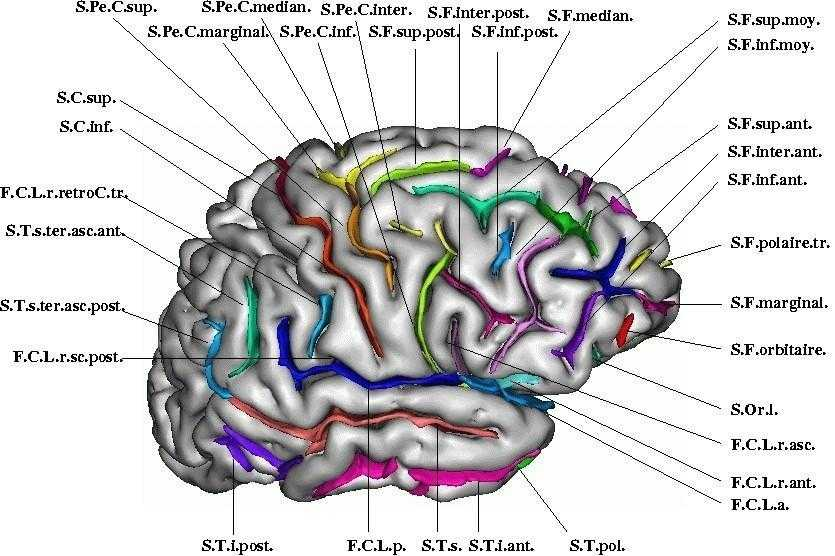
\includegraphics[width=12cm, height=7.5cm]{vuescerv.jpg}
    \caption{\textit{Schéma du plissement cérébral}}
    \label{fig:cerveau}
\end{figure}

\vspace{5mm}

Le mécanisme de formation des plis est toujours un sujet de recherche actif et plusieurs théories existent. Ils pourraient ainsi être le résultat d’une simple compression mécanique permettant d'accroître la surface du cerveau. Une autre hypothèse est liée à des considérations génétiques. Cependant, les cerveaux pliés ne sont pas la norme dans le règne animal. Le cortex des souris et des rats par exemple, ne s’agrandit pas suffisamment au cours du développement pour conduire à ce “pliage” : leurs cerveaux présentent ainsi des surfaces complètement lisses.

Chez l'humain, l'étude de ceux-ci peut se révéler extrêmement utile comme l'a montré une étude publiée en 2019 \cite{bertoux_sulcal_2019}. L'analyse des sillons, et plus précisément leur largeur est un nouveau marqueur de la maladie d'Alzheimer.

Ainsi, notre étude s'inscrit dans un secteur de recherche actif et fondamental pour la compréhension de notre fonctionnement. Aujourd'hui, les nouvelles méthodes d'analyse d'images à l'aide du \textit{machine learning}, ainsi que les nouvelles ressources computationnelles à notre disposition ouvrent la voie à cet approfondissement. 

\subsection{Synthèse}

\vspace{5mm} 

Le but du stage est, en explorant les différents types de \textit{Generative Adversarial Networks} (GAN), de capturer cette variabilité intra-humaine. Pour ce faire, on donne aux GANs la tâche de générer des images de cerveaux sains.

\vspace{5mm} 

Les résultats du stage ont pour but d’être utilisés dans un projet de détection d’anomalies cérébrales de ma tutrice Louise Guillon. En effet, si l’on arrive grâce aux GAN à capturer la variabilité humaine des sillons cérébraux, le dispositif pourrait donc, avec une image de cerveau en entrée, calculer un distance entre sa modélisation de cerveaux apprise et l’encodage du cerveau et donc en conclure s'il y a ou non une anomalie. 

\vspace{5mm} 

Durant mon stage, j’ai été amené à travailler sur 2 projets, un projet préliminaire qui avait pour but de me familiariser avec les outils de Neurospin, et mon projet principal qui est donc mon sujet de stage. Le langage de programmation est \textit{Python} et j'ai principalement travaillé avec les librairies Pytorch, librairie standard de \textit{Deep Learning}, et AIMS (\textit{"Analysis of Images and Signals"}), librairie du projet \textit{BrainVisa} développé dans le laboratoire d'accueil.
Le premier projet avait pour but d’implémenter quelques réseaux de neurones trouvés dans la littérature afin de transformer en une image de squelette de cerveau, qui représente uniquement les plissement de la matière cérébrale, en une image de segmentation de la matière blanche et de la matière grise, c'est-à-dire correspondant à peu près à ses contours, une IRM de cerveaux déchargée de certaines informations et qui comporte un nombre restreint de niveaux de gris différents.
Pour ce faire, j’ai implémenté 2 structures différentes que j’ai choisies suite à mon étude de l’état de l’art: Le Unit (\textit{Unsupervised Image-to-Image Translation Networks}) \cite{liu_unsupervised_2018} et le VNET (\textit{Volumetric Network}) \cite{milletari_v-net_2016}. Le premier repose conjointement sur les concepts de GAN et d’auto-encodeur (AE), le second repose sur le même concept que le Unet \cite{ronneberger_u-net_2015} mais pour des volumes, un réseau avec une phase descendante de modélisation des données, et une phase ascendante permettant la reconstruction dans le domaine des images. Ces structures seront développées dans la suite du rapport.

\vspace{5mm} 

Les résultats du Unit n'ont pas été satisfaisants. En effet, la recherche de paramètres n'a pas permis de trouver de bonne combinaison, sûrement du fait de la forte complexité du modèle, ou alors du fait d'une architecture non adaptée à nos données.
De son côté, le Vnet est initialement destiné à de la segmentation de volumes mais on peut adapter la fonction objectif comme on le souhaite. Ici on l’utilise donc pour transformer des images de squelettes en images de segmentation matière blanche-matière grise. Avec cette architecture, nous arrivons à des résultats très satisfaisants comme nous le verrons dans sa partie dédiée V.2.4. Il est fort possible qu’avec une étude plus poussée, le Vnet réponde totalement à la demande. Néanmoins, je n’ai pas poussé cette étude jusqu'à la fin car, n'étant pas mon sujet principal de stage, nous avons décidé de clôturer celui-ci.

\vspace{5mm} 

Je me suis ensuite concentré sur les GAN, en étudiant le Wasserstein GAN \cite{arjovsky_wasserstein_2017}, le Deep Convolutional GAN (ou dcGAN) \cite{radford_unsupervised_2016} et enfin le wGAN-gp (gp pour Gradient Penalty) \cite{gulrajani_improved_2017}. Le but de ce projet était de se concentrer sur les squelettes de cerveaux. Nous verrons ensuite leurs spécificités, mais il est important de noter que j’ai graduellement essayé des modèles de plus en plus complexes, et de moins en moins classiques pour répondre au problème posé. Avec raffinement successif du modèle, je suis arrivé à un modèle répondant aux exigences, composé classiquement d’un générateur et d’un discriminateur, mais aussi d’un encodeur. Ce modèle, hybride entre un GAN classique et un auto-encodeur, a permis dans un premier temps la bonne reconstruction du squelette donné en entrée, puis a vérifié de bonnes propriétés lors de l’étude de son espace latent (espace de plus petite dimension dans lequel sont projetées les images d’entrée).


\newpage
\section{Présentation de l’entreprise}


\subsection{Présentation générale}

Le Commissariat à l’énergie atomique et aux énergies alternatives (CEA), créé le 18 octobre 1945 par Charles de Gaulle avec à sa tête Frédéric Joliot-Curie (haut-commissaire à l’Énergie atomique) et Raoul Dautry (administrateur général), est un organisme public de recherche à caractère scientifique, technique et industriel. Acteur majeur de la recherche, du développement et de l'innovation, le CEA intervient dans quatre domaines : la défense et la sécurité, les énergies bas carbone (nucléaire et renouvelables), la recherche technologique pour l'industrie et la recherche fondamentale (sciences de la matière et sciences de la vie). S'appuyant sur une capacité d'expertise reconnue, le CEA participe à la mise en place de projets de collaboration avec de nombreux partenaires académiques et industriels. L’organisme fût créé en septembre 1945 lorsque le général de Gaulle demande au directeur du CNRS Frédéric Joliot-Curie et à Raoul Dautry, alors ministre de la reconstruction et de l'urbanisme, de mettre en place un organisme de recherche consacré à l'énergie atomique. 

\vspace{5mm} 
 Cet organisme est placé sous l’autorité directe de la présidence du Conseil, ses finances ne faisant l’objet que d’un contrôle \textit{a posteriori} par le ministère des Finances. Les principales données de ressources et de dépenses du rapport financier de 2020 sont présentées en annexe 1 et 2.

\vspace{5mm} 
J'ai eu la chance de faire mon stage au sein de NeuroSpin, un centre de recherche en imagerie cérébrale et neurosciences, localisé sur le campus public du centre CEA de Saclay, inauguré en 2007. Les travaux menés s’articulent autour de deux directives principales : l’innovation en neuro-imagerie par IRM à ultra haut champ magnétique et son utilisation en recherche biomédicale et neurosciences cognitives pour une meilleure compréhension du cerveau sain et malade. Mon stage prend spécifiquement place au sein de l'équipe BAOBAB \textit{(Building large instruments for neuroimaging: from population imaging to ultra-high magnetic fields}), sous la tutelle du CEA, du CNRS et de l'université Paris Saclay. Cette équipe est née de la fusion de deux Unités de recherche UNIRS et UNATI. Un organigramme des équipes est en annexe 3.


\subsection{Bilan général sur la responsabilité sociétale et environnementale (RSE)}

\subsubsection*{Volet environnemental}

Le CEA place le développement durable au cœur de ses préoccupations, en cherchant à réduire l’empreinte environnementale de ses activités de R\&D tout en favorisant leur bénéfice économique et le bien-être de ses salariés. Coordonnées au niveau national, ces actions sont soutenues, au niveau des territoires, par des initiatives conduites par chaque centre en fonction de ses spécificités.  On peux noter deux actions phares qui ont été menées en 2019 par le CEA, détaillées sur leur site web.
\begin{itemize}
    \item La première concerne la réduction de 3 \% de sa consommation énergétique. Sur la base de l’audit énergétique réglementaire de ses installations finalisé en 2019, le CEA a lancé le projet « performance énergétique » pour la période 2020-2023, avec trois objectifs principaux : établir la politique énergétique de l’organisme, adapter l’organisation et les processus des activités d’exploitation, de maintenance et de rénovation à la recherche de performance énergétique dans la durée et poser la méthodologie de réduction des consommations énergétiques de 3 \% par an à périmètre constant.

Parallèlement, il a continué son effort de réduction, de verdissement et de rajeunissement de son parc automobile, composé de 494 véhicules (en réduction significative tous les ans). En termes de motorisation, la part du diesel qui s’élevait à 43 \% du parc automobile en 2017 ne représente plus que 30 \% en 2019 alors que la part de motorisation électrique et hybride atteint 40 \% en 2019 (33 \% en 2017). 
    \item La deuxième action engagée en 2019 porte sur la responsabilité dans les achats. Le CEA a ainsi réalisé une analyse fine de la consommation de ses déchets plastiques, plus particulièrement des gobelets utilisés quotidiennement par ses salariés (environ 25 tonnes par an, avec un impact environnemental non négligeable). Fort de ce constat et suite à la promulgation des lois sur la transition énergétique et l’économie circulaire, le CEA a fait le choix de produits lavables (verres, tasses) associés à des solutions de nettoyage par la restauration, le service nettoyage ou l’achat de machines de lavage portables, qui constituent le meilleur compromis économie/environnement.
\end{itemize}


\subsubsection*{Volet sociétal}
Peu d’information concernant la politique sociale du CEA sont disponibles. J’ai tout de même remarqué que l’on y retrouve un très grande mixité sociale, au sein d’un même bâtiment de nombreux pays sont représentés. Au sein de NeuroSpin, je n’ai pas remarqué de déséquilibre en terme de présence entre les hommes et les femmes. Dans certaines équipes les femmes sont même parfois plus nombreuses que les hommes. La principale observation que j’ai faite est que les postes permanents sont majoritairement occupés par des hommes et les femmes sont plus souvent des doctorantes. 


\vspace{5mm} 

\subsection{Santé et sécurité}

\vspace{5mm} 

La première priorité du CEA est de maîtriser les risques inhérents aux installations nucléaires nécessaires à ses activités de recherche. La sécurité et la sûreté sont, en effet, déterminantes pour protéger le personnel, le public et l'environnement.  
L'affirmation de cette priorité influence l'ensemble des activités et l'organisation du CEA en plaçant cet impératif au cœur des préoccupations de chacun. Elle s'impose tout particulièrement aux réacteurs de recherche, laboratoires et centres de traitements des effluents et déchets utiles aux recherches du CEA. Un effort continu de minimisation de la production de déchets et de réduction des rejets dans l'environnement accompagne un programme soutenu d'amélioration de la qualité des installations et d'assainissement et démantèlement des installations obsolètes.

\vspace{5mm} 

Le domaine de l'hygiène et de la sécurité du travail (risque incendie, risque électrique, risque chimique et biologique, risque lasers...) s'intègre dans cette préoccupation et fait l'objet de programmes d'actions spécifiques.


\newpage


\section{État de l’art}

\vspace{5mm} 

La première partie de cette revue de l'état de l'art se consacre aux GAN et à leurs variantes principales. Ensuite, des réseaux faisant du \textit{"image-to-image translation"} sont décrits. Enfin, nous verrons comment les GANs sont déjà utilisés dans le domaine médical et à quelles fins.

\vspace{5mm} 


\subsection{GAN}
 
 \vspace{5mm} 
 Les GANs (\textit{Generative Adversarial Networks}) sont des types d’architectures reposant sur la compétition entre un réseau générateur, qui a pour tâche de créer des images plausibles, et un discriminateur dont le but est d’apprendre à discerner les images réelles des images générées par le générateur \cite{goodfellow_generative_2014}. Ils sont utilisé notamment pour de l'augmentation de données, de la classification et ont même contribué à l'essor des \textit{deep fakes}, permettant de mettre en scène des personnalités dans toutes sortes de situations de manière extrêmement réaliste. Pour cela, il donne en sortie la probabilité que l'image donnée soit réelle. L'entrée du générateur est un bruit, c'est-à-dire une matrice aléatoire, d'une certaine dimension que l'on peut choisir. 
 
Un an après, apparaît une version plus performante du GAN, le dcGAN. Le réseau antagoniste génératif convolutif profond, ou dcGAN, est une extension de l'architecture GAN permettant d'utiliser des réseaux neuronaux convolutifs profonds pour les modèles du générateur et du discriminateur qui aboutit à l'entraînement plus stable d'un modèle de générateur \cite{radford_unsupervised_2016}.
 
 Le GAN classique, \textit{via} son générateur permet la génération d'images nouvelles, mais comme son entrée est du bruit, nous ne donnons aucune restriction sur ses productions. Les réseaux adversaires peuvent être étendus à un modèle conditionnel si le générateur et le discriminateur sont tous deux conditionnés par une information supplémentaire y. C'est le principe du \textit{conditional} GAN (cGAN), décrit en 2014, qui permet de mieux maîtriser les générations du modèle \cite{mirza_conditional_2014}. L'information supplémentaire est en général un vecteur que l'on donne au générateur et au discriminateur conjointement à leurs entrées de base en les concaténant. On travaille alors avec des probabilités conditionnelles.
Le cGAN est efficace pour des tâches peu complexes comme avec la base de donnée classique MNIST (qui contient des chiffres écrits à la main sur fond noir). Il est meilleur que le GAN classique et converge plus vite. Néanmoins, cette efficacité peine à être retrouvée pour des tâches plus complexes. 

En 2017 est publié un article fondateur dans les travaux sur les GANs. Écrit plutôt comme une démonstration mathématique, les auteurs proposent le Wasserstein GAN qui introduit une subtile modification au concept de GAN \cite{arjovsky_wasserstein_2017}. En effet, ils modifient la procédure d'apprentissage pour mettre à jour  à chaque itération le modèle discriminateur, désormais appelé critique, contrairement au générateur, qui sera mis à jour par exemple toutes les trois ou quatre époques. Le critique est modifié pour produire une valeur réelle au lieu d'une prédiction binaire, et les modèles du critique et du générateur sont tous deux entraînés en utilisant la "distance de Wasserstein" (qui sera davantage expliquée dans la section V.2.2). 

 
\subsection{Image-to-image-translation}


L'\textit{image-to-image translation} ou translation d'image est un domaine de recherche en \textit{machine learning} qui étudie la tâche consistant à prendre des images d'un domaine et à les transformer pour qu'elles aient le style (ou les caractéristiques) d'images d'un autre domaine. On peut par exemple transformer une image comportant un cheval en une image avec un zèbre. Pix2pix apprend ce type de tâche de manière supervisée en utilisant des cGAN \cite{isola_image--image_2018}. Il combine une méthode antagoniste avec une régularisation L2, ce qui nécessite des échantillons de données appariés. Pour pallier au problème de l'obtention de paires de données, des modèles non-supervisés ont été mis au point. 

Un modèle important dans cette thématique de traitement d’images est le Unit (\textit{Unsupervised Image-to-Image Translation Network}) \cite{liu_unsupervised_2018} car il est très novateur dans son approche. Le but de ce modèle est d’apprendre une fonction liant deux domaines différents (par exemple transformer une image de chat en chien et inversement). Le Unit propose une architecture entre le GAN classique et l’autoencodeur qui permet d’apprendre une distribution conjointe des deux domaines. Ce modèle sera utilisé dans le projet n°1 et nous verrons qu’il a ses limites, dont le fait qu’il ne puisse représenter que deux domaines. 

Le StarGAN \cite{choi_stargan_2018}, modèle proposé en 2018, répond à ce problème en proposant un modèle proche du cGAN, en donnant conjointement l’image source et une étiquette conditionnant la génération, ou plutôt la transformation de l'image. Cependant, StarGAN a été fortement critiqué pour son manque de généralisation. En effet, le modèle a du mal à diversifier ses images générées et ne permet pas de capturer la variabilité des différentes images d'un même domaine. La version 2 de StarGAN \cite{choi_stargan_2020} a été développée en 2020 pour répondre à cette problématique. Il permet de capturer cette variabilité en ajoutant un 'encodeur de style' . 

\subsection{Application de modèles génératifs dans le domaine médical}

 
Enfin, nous allons voir les applications de ces modèles de \textit{machine learning} dans le domaine médical car c'est dans ce contexte que se situent mes projets. Les progrès dans la reconnaissance de motifs par apprentissage automatique sont cruciaux dans ce domaine et constituent un énorme enjeu pour le futur. 

Par exemple, l'avènement des réseaux convolutifs a énormément fait avancer la recherche et a notamment fait émerger le réseau Vnet \cite{milletari_v-net_2016}. Les auteurs y proposent une approche de
segmentation d'images 3D fondée sur un réseau de neurones volumétrique, entièrement convolutif. Le réseau est entraîné sur des volumes IRM représentant la prostate et apprend à prédire la segmentation de l'ensemble du volume en une seule fois. 
Une autre application majeure du \textit{deep learning} dans le domaine médical est la détection d'anomalies. C'est le but de l'AnoGAN, présenté en 2017 \cite{schlegl_unsupervised_2017}. Les auteurs proposent un apprentissage non supervisé pour identifier les anomalies dans les données d'imagerie en tant que candidats pour des nouveaux marqueurs de maladies. Le réseau développé est un réseau convolutif génératif antagoniste profond. L'objectif est d'apprendre la variabilité anatomique "normale". Ils introduisent également un nouveau score d'anomalie basé sur le mapping de l'espace des images à un espace latent. Appliqué à de nouvelles données, le modèle étiquette les anomalies et note les parties d'images en fonction de leur adéquation avec la distribution apprise. 

Bien que l'AnoGAN ait montré de bonnes performances en matière de détection d'anomalies, ce réseau est très coûteux en terme de ressources computationnelles et est finalement peu efficace car il repose sur des mécaniques itératives qui convergent trop lentement. La technique f-AnoGAN \cite{schlegl_f-anogan_2019} remplace cette procédure itérative par un mapping appris de l'image à l'espace latent, ce qui améliore considérablement la vitesse. 

Il est également important de parler du problème du déséquilibre des données médicales, c'est-à-dire que, pour une pathologie donnée, nous ne disposons pas du même nombre d'images pour toutes les sous-pathologies de celle-ci, ce qui rend son étude compliquée. Dans un article publié en 2019, les auteurs proposent un WGAN pour répondre à cette problématique \cite{wang_wgan-based_2019}. Le WGAN peut estimer la distribution sous-jacente d'une classe minoritaire afin de synthétiser des échantillons plus plausibles et utiles pour le modèle de classification. La technique de sur-échantillonnage basée sur le WGAN est appliquée pour augmenter le nombre d'images à dispositions. Cela à pour but d'équilibrer les bases de données pour la classification de sept attributs sémantiques de nodules pulmonaires dans des images de tomographie par ordinateur. 

Enfin, la synthèse d'images via les GANs a un grand potentiel  qui peut être étendu à de nombreuses applications médicales, telles que l'amélioration de résolution des images médicales et la modélisation de la progression des maladies. Ainsi, très récemment,  3D-StyleGAN a été développé afin de répondre à cette problématique \cite{hong_3d-stylegan_2021}.


\newpage

\section{Données et pré-traitements}

\subsection{Données}
Lors des différents projets, j'ai été amené à travailler sur des images d'IRM-t1 de la base de données publique HCP (\textit{Human Connectome Project}). Elle contient des données cérébrales de plus de 1000 sujets. Le HCP cartographie le cerveaux humains sains en collectant et en distribuant librement des données de neuro-imagerie et de comportement sur 1 200 jeunes adultes contrôles, âgés de 22 à 35 ans. Les images peuvent être visualisées à l'aide d'outils de BrainVisa, logiciel en accès libre développé par l'équipe. 


\begin{figure}[H]
    \centering
    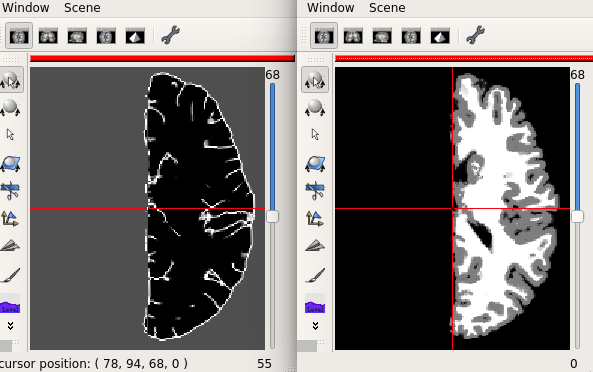
\includegraphics[width=10cm, height=6cm]{hcp.png}
    \caption{\textit{Coupe d'un sujet du HCP vue avec les outils de BrainVisa: à gauche un squelette et à droite une image gris-blanc}}
    \label{fig:anatomist}
\end{figure}

\vspace{5mm} 
Les IRM cérébrales contiennent diverses informations qui ne sont pas toutes pertinentes pour étudier les modèles de plissement. Afin de pouvoir utiliser ces images d'IRM, il est important de normaliser les images car elles sont dans l'espace natif du sujet et spécifiques au scanner IRM. On ne peut donc pas comparer les données entre elles les coordonnées n'étant pas superposables. On va alors utiliser une \textit{pipeline} pour répondre à ce problème.\\

\subsection{Morphologist, logiciel de pré-traitement standard des images IRM}

Durant 6 mois, j'ai principalement travaillé avec des images de squelettes de cerveaux. Les images de squelettes de cerveaux sont des images 3D représentant des surfaces médiales aux plissements, qui ressemblent aux feuillets que l’on découvre parfois dans les plis des noix. Ces images   sont   obtenues   à   partir   d’une   chaîne   de   traitements   développée   au   sein   de   l’équipe (http://brainvisa.info). En effet, BrainVisa fournit une infrastructure complète et modulaire pour les images de neuro-imagerie. Il permet d'organiser des logiciels et des données hétérogènes et fournit une interface graphique générale commune aux utilisateurs. C'est donc un ensemble d'outils plutôt qu'un logiciel unique. Ci-dessous figure \ref{fig:anatomist}, une visualisation de nos données de départ avec le logiciel Anatomist de BrainVisa.

Notre méthode comprend donc une première étape cruciale de pré-traitement des données, qui passent dans une \textit{pipeline}. Cette \textit{pipeline} combine plusieurs étapes telles que la correction de biais, la ségrégation gris-blanc et la squelettisation afin d'obtenir une image négative du plissement. Le résultat est un volume 3D avec trois valeurs : intérieur du cerveau, squelettes des sillons et extérieur du cerveau. L'utilisation de ces images simples plutôt que des IRM brutes permet de concentrer l'apprentissage sur la géométrie de plissement et écarte certains biais (comme le biais dû à l'âge, le vieillissement s'accompagnant d'un élargissement des plis, ou le biais dû au centre dans lequel a été faite l'IRM). \\


\subsection{Pré-traitements supplémentaires}
Une fois les images de squelettes et gris-blanc, par simplicité, les images de segmentation de matière blanche-matière grise seront appelées "gris-blanc", obtenues grâce à Morphologist, plusieurs étapes supplémentaires de pré-traitement sont nécessaires et notamment un sous-échantillonage. En effet, il n'est pas nécessaire de travailler avec des images de résolution extrêmement élevée. Nos images de base ont une résolution de 0.7mm par voxel (cube Unité, pixel volumique), ce qui est relativement élevé, nous sommes donc passés à une résolution de 1mm, et dans certains cas 2mm. Pour ce faire, différentes techniques sont possibles dont: 
\begin{itemize}
\item \textbf{Max pooling}: En considérant que l'on veuille diminuer la taille par 2, il suffit, pour chaque carré de 4 pixels, de garder la valeur maximale;
\item De même, on peut penser à la technique du \textbf{plus proche voisin} où l'on réduit un ensemble de pixels à la valeur de son pixel le plus central;
\item On utilise aussi \textbf{l'interpolation linéaire} : On moyenne la valeur des pixels voisins et on attribue au pixel résultant la valeur la plus proche parmi l'ensemble des valeurs d'origines;

\item Néanmoins, ces techniques, bien que classiques, ne sont pas bien adaptées pour notre problème. En fait, en procédant ainsi nous risquons de supprimer certaines parties de sillons, les rendant morcelés et nous perdons ainsi de l'information cruciale. Nous avons donc finalement opté pour un sous-échantillonage de type \textbf{plus proche voisin mais en mettant une priorité sur les sillons}. Ce sous-échantillonage marche comme ci-dessus mais permet en plus de garder les sillons intacts et continus.
\end{itemize}

Ensuite, il faut couper les bords noirs, alors inutiles pour notre étude. Pour cela, on recherche le \textit{crop} minimal, c'est-à-dire la taille minimale de l'image telle que tous les cerveaux du HCP soient compris dedans, tout en enlevant le maximum de partie noire. Après cette recherche, on passera d'images de taille de (260, 311, 260) voxels à des images d'une taille de (135, 185, 85) voxels, puis (192, 192, 192) voxels lorsqu'on a décidé de passer à des images 3D cubiques ce qui simplifiera l'architecture des réseaux utilisés ensuite. Dans certains réseaux, il s'ensuit un sous-échantillonnage par 2, réduisant les images à une taille de (43,96, 83) voxels et de (96,96,96) voxels pour les images cubiques. \\

Enfin, il faut transformer ces images en données exploitables par un réseau de neurones.
Pour ce faire, on met les données sous forme de tableaux que l'on enregistre en fichiers Pickle. On convertit ensuite les tableaux de données en tenseurs de taille (nombre de sujets, nombre de canaux (1 ici), (taille de l’image) ) et on crée des ensembles de train, validation et test, selon la taille de \textit{batch} (taille d'un groupement de sujets), paramètre modulable. Ci dessous figure \ref{fig:prepro} le résultat du pré-processing pour une image gris-blanc.\\

\begin{figure}[H]
    \centering
    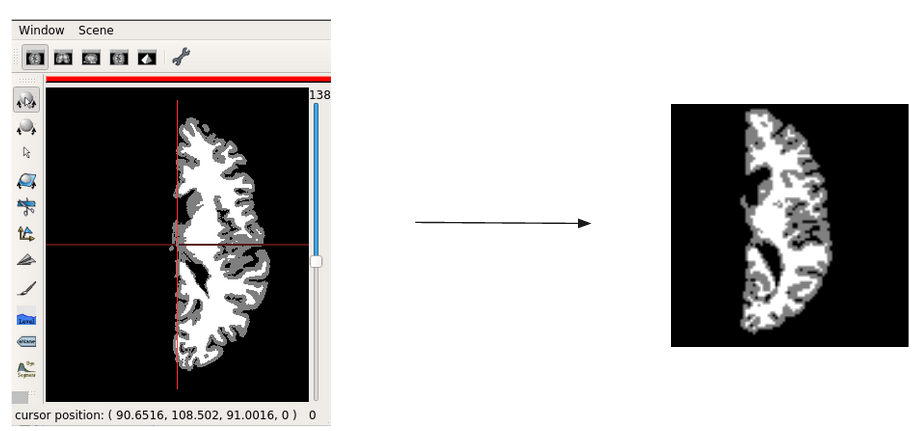
\includegraphics[width=12cm, height=5cm]{prepro.png}
    \caption{\textit{Résultat du préprocessing pour une image gris-blanc}}
    \label{fig:prepro}
\end{figure}

À noter que les images d'entrées ne sont pas toujours cubiques dans mes modèles car ce n'est qu'a partir du modèle du Vnet que j'ai commencé à travailler avec des volumes de même taille sur les 3 dimensions pour faciliter les architectures.



De même, jusqu'au Vnet, le travail était fait avec la technique de sous-échantillonage d'interpolation linéaire durant le pré-traitement, qui était le paramètre par défaut. Cette technique crée de nouvelles valeurs pour les images traitées alors que nous travaillons sur un ensemble réduit dès le départ. Pour faciliter l'apprentissage, on binarise les images de squelettes et de réduire à 3 valeurs les images en gris-blanc. Pour ce faire, les valeurs des voxels sont remplacées par leur valeur la plus proche parmi \{0,1\}, sillon ou pas sillon, pour les images de squelettes et \{0,100,200\}, correspondant aux parties blanches, grises et noires pour les images en gris-blanc comme vu figure 2.



Ci-dessous figure \ref{fig:recap}, un récapitulatif des données utilisées et générées avec les différentes architectures.



\begin{figure}[H]
    \centering
    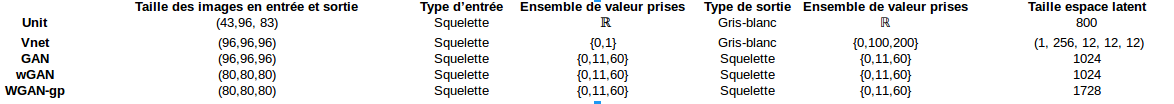
\includegraphics[width=14cm, height=2cm]{recap.png}
    \caption{\textit{Tableau récapitulatif}}
    \label{fig:recap}
\end{figure}


À noter que pour le Vnet, la dimension de l'espace latent n'est pas un nombre car nous verrons section V.1.2 que dans ce cas précis, on n'encode pas en un vecteur les images mais on ne fait que réduire la résolution itérativement. La taille dans cette case correspond donc à la taille de la plus petite image.



\newpage

\section{Modèles et implémentations}

\subsection{Projet n°1 : des images de squelettes à des images gris-blanc}

Nous allons maintenant détailler les deux projets auxquels je me suis attelé durant le stage. Pour ceux-ci, j'ai pu avoir accès à KRAKEN, un ensemble de GPUs dédiés aux calculs pour le \textit{deep learning}. Cette connexion a pu être effectuée à distance durant les pics d'épidémie de Covid-19 par VPN. \\

\vspace{5mm} 

J'ai commencé par travailler sur un projet intermédiaire afin de prendre en main les données du HCP et de me familiariser avec les outils de l'équipe. Le but de ce premier projet est de développer un modèle permettant de transformer une image de squelette de cerveau en une image gris-blanc, comprenant plus de valeurs différentes et donc plus d'informations. Pour ce projet et une partie du deuxième projet, nous nous sommes intéressés uniquement à l'hémisphère gauche. Ci-dessous la figure \ref{fig:proj1} présente un exemple d'une coupe de cerveaux en squelette puis en gris-blanc comme devrait le faire le modèle :

\begin{figure}[H]
\centering
\begin{subfigure}{.2\textwidth}
  
\includegraphics[width=\textwidth]{X1_3330.png}
  \caption{Squelette}
  \label{fig:sub1}
\end{subfigure}%
\begin{subfigure}{.2\textwidth}
  
\includegraphics[width=\textwidth]{X2_3330.png}
  \caption{Grey white}
  \label{fig:sub2}
\end{subfigure}
\caption{\textit{Coupe d'un cerveau en squelette à gauche et en gris-blanc à droite}}
\label{fig:proj1}
\end{figure}

\vspace{5mm}

Suite à l'état de l'art, j'ai décidé de retenir 2 modèles pour ce projet. En effet, ils ont tout deux prouvé leur efficacité sur d'autres bases de données. Le premier reprend les mécaniques des GAN, ce qui me semblait être formateur pour la suite du stage, et le second a été retenu suite aux limites du premier.

\subsubsection{Unit}

Le tout premier modèle auquel je me suis intéressé lors de ce stage est le Unit \cite{liu_unsupervised_2018}. Je l'ai choisi car il semblait très prometteur et proposait une infrastructure innovante et croisant plusieurs concepts. En effet, le modèle repose sur un système de couplage de deux GANs et d'un VAE (\textit{Variational Auto-Encoder}) avec un partage de poids aux dernières couches de l'encodeur et aux premières couches du décodeur comme sur la figure ci-dessous. E désigne les encodeurs, G les générateurs et D les discriminateurs. Leur numéro correspond au domaine auquel ils sont rattachés (G1 désigne le générateur qui produit des images dans le domaine 1, E2 l'encodeur qui encode des images du domaine 2 dans l'espace latent...). Le fonctionnement d'un GAN sera explicité en profondeur dans le projet n°2.

\begin{figure}[H]
    \centering
    \includegraphics[width=9cm, height=4cm]{Unit.png}
    \caption{\textit{Structure du Unit}}
    \label{fig:Unit}
\end{figure}
\vspace{5mm}
Le fonctionnement de la transformation d'une image d'un espace à un autre est assuré par espace latent partagé: une paire d'images correspondantes dans différents domaines peut être mise en correspondance avec une même représentation latente dans un espace latent partagé. En effet, puisqu'il existe un ensemble infini de distributions conjointes à partir des distributions marginales données, on ne peut rien en déduire sans hypothèses supplémentaires.
Le principe fondamental de cette architecture est que, pour chaque paire d'images x1 et x2, respectivement dans leur domaine X1 et X2, il est possible de les projeter au même point par encodage dans l'espace latent.
\begin{figure}[H]
    \centering
    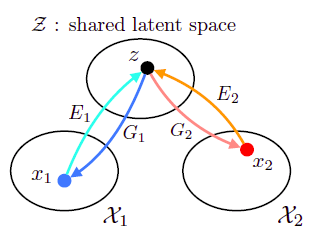
\includegraphics[width=6cm, height=4cm]{shared.png}
    \caption{\textit{Schéma du partage du code latent }}
    \label{fig:code}
\end{figure}


L'autre principe phare du modèle est son système de partage de poids, modélisé dans la figure \ref{fig:Unit} par des lignes pointillées. Cette technique limite la capacité du réseau et favorise une solution de distribution conjointe plutôt qu'un produit de distributions marginales \cite{liu_unsupervised_2018}.

Enfin la fonction objectif de ce module se formule comme ci-dessous:
\begin{equation}
   \min_{E_{1},E_{2},G_{1},G_{2}} \max_{D_{1},D_{2}}\mathcal{L}_{VAE_{1}}(E_{1},G_{1}) + \mathcal{L}_{VAE_{2}}(E_{2},G_{2})+ \mathcal{L}_{GAN_{1}}(E_{2},G_{1},D_{1})+
    
    \mathcal{L}_{GAN_{2}}(E_{1},G_{2},D_{2})+\mathcal{L}_{CC_{1}}(E_{1},G_{1},E_{2},G_{2})+\mathcal{L}_{CC_{2}}(E_{2},G_{2},E_{1},G_{1})
\end{equation}

\vspace{5mm}

 Ce qui est important à comprendre de la fonction objectif est qu'elle comporte 3 pertes différentes: une modélisant la perte des GAN (elle sera explicitée dans le projet suivant), le premier étant composé de E2, G1 et D1; une autre modélisant celle des VAE (\textit{Variational Auto-Encoder}) de chaque domaine que l'on ne détaillera pas; et enfin une annotée 'CC' pour \textit{cycle consistency} qui modélise la qualité d'une image encodée dans l'espace latent puis re-générée dans son espace de départ, formant alors un cycle (c'est une perte de reconstruction).\\

Pour appliquer ce modèle à notre problème de transformation d'images squelettes de cerveau à des images gris-blanc, j'ai alors constitué des paires d'images de chaque ensemble et chaque sujet, pré-traitées comme expliqué précédemment. La première difficulté a été d'adapter ce modèle, initialement prévu pour des images 2D, en 3D. Il a donc fallu adapter toutes les couches du modèle en utilisant les outils à disposition sur \textit{Pytorch}.

\subsubsection{Vnet}
Le deuxième modèle développé est le Vnet, une version volumétrique du Unet qui avait déjà fait ses preuves dans de nombreux domaines de traitement d'images \cite{milletari_v-net_2016}. Ce modèle a l'avantage d'être moins complexe et plus adaptable. L'Unet \cite{ronneberger_u-net_2015} est utilisé pour la segmentation d'images bio-médicales. L'architecture contient deux composantes. Le premier est le chemin de contraction (également appelé l'encodeur) qui est utilisé pour capturer le contexte dans l'image. L'encodeur est une succession de couches convolutionnelles. Le deuxième chemin est le chemin d'expansion symétrique (également appelé décodeur) qui est utilisé pour permettre une localisation précise en utilisant des convolutions transposées. Il s'agit donc d'un réseau entièrement convolutif, c'est-à-dire qu'il ne contient que des couches de convolution et aucune couche dense, ce qui lui permet d'accepter des images de toute taille. L'architecture du Vnet est présenté figure \ref{fig:Vnet}.

\begin{figure}[H]
    \centering
    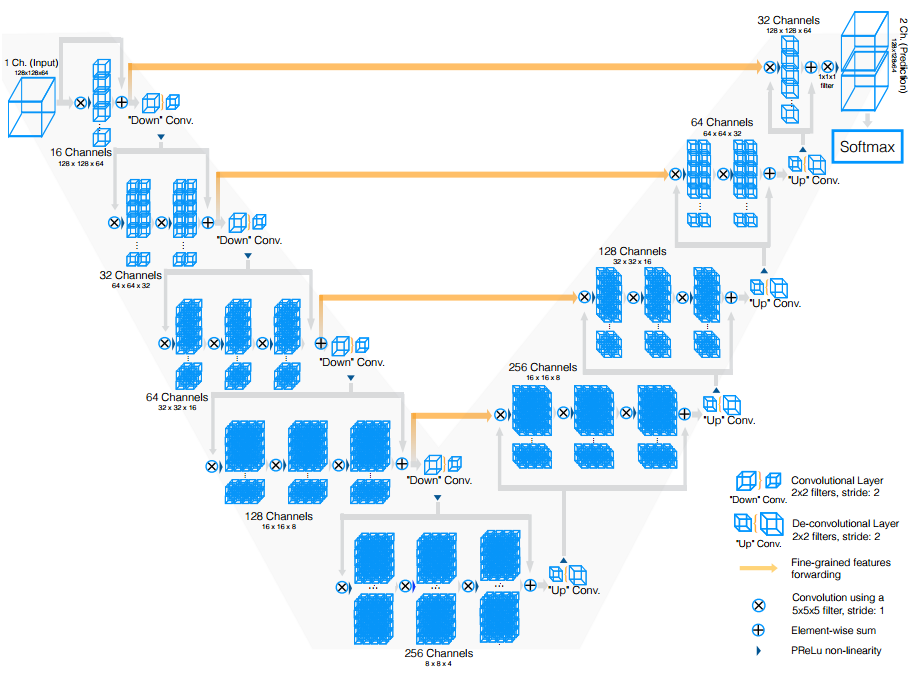
\includegraphics[width=9cm, height=8cm]{vnet.png}
    \caption{\textit{Schéma de l'architecture du Vnet}}
    \label{fig:Vnet}
\end{figure}


\vspace{5mm}

Dans l'article original, les auteurs introduisent la 'DICE loss', optimisée pour de la segmentation sémantique et des images où il y a une grande différence de surface entre le premier plan, avec les objets d'intérêts, duquel on souhaite détacher de l'arrière plan. Dans notre cas, nous travaillons avec des images de squelettes et des images gris-blanc avec un nombre limité de valeurs. C'est pourquoi on remplace la perte par une \textit{cross-entropy} à trois valeurs, ce qui facilite énormément l'apprentissage. J'ai modifié en conséquence la sortie du générateur pour qu'il ressorte la probabilité d'appartenance à une des trois classes étant donné l'image en squelette binarisé. 

\vspace{5mm}

Le Vnet étant alors adapté, j'ai lancé l'entraînement sur le répertoire du HCP. J'ai été confronté à la limitation de la mémoire GPU sur le serveur distant. J'ai alors été contraint de réduire le nombre de sujets d'entraînement à 100 cerveaux au lieu de 1000. De plus, j'ai ajouté un système de sauvegarde des modèles. En effet, étant connecté en VPN sur le serveur distant, des entraînements trop longs ne sont pas possibles car il y a un risque d'interruption de la connexion ce qui annulerait tout l'entraînement. Ainsi, je n'ai lancé que des entraînements relativement courts de maximum 50 époques, suivis d'un enregistrement du modèle et ceci en boucle.

\vspace{5mm}

\subsubsection{Résultats}

\vspace{5mm}

\textbf{Unit} \\

\vspace{1mm}

Lors de ce projet j'ai été confronté à un problème majeur et récurrent à savoir la gestion de la mémoire GPU. 
En effet, je travaille sur un GPU distant de 48601 MiB de RAM (mébioctets, 1MiB = \(2^{20}\) octets) ce qui me limite dans les paramètres choisis des infrastructures comme le nombre de filtres pour les couches convolutionnelles ou le nombre de couches au total, et les calculs. Le modèle Unit comme décrit dans l'article et avec les adaptations pour gérer des images 3D, dépasse largement les caractéristiques d'un GPU de KRAKEN.
J'ai donc largement vu à la baisse l'architecture en modulant certains paramètres, en baissant par exemple le nombre de filtres des couches convolutionnelles les plus basses et certaines couches ont été supprimées.
De fait, j'ai dû aussi modifier le pré-traitement en ajoutant un sous-échantillonage par deux des images d'entrée.

\vspace{5mm}

Le modèle a finalement tourné sur le serveur distant mais n'est pas parvenu à apprendre comme le montre la figure \ref{fig:res_Unit}. Il semble que les générateurs n'ont pas réussi à apprendre la variabilité des domaines et que le discriminateur arrivait très facilement à discerner les images réelles des générées.

\begin{figure}[H]
    \centering
    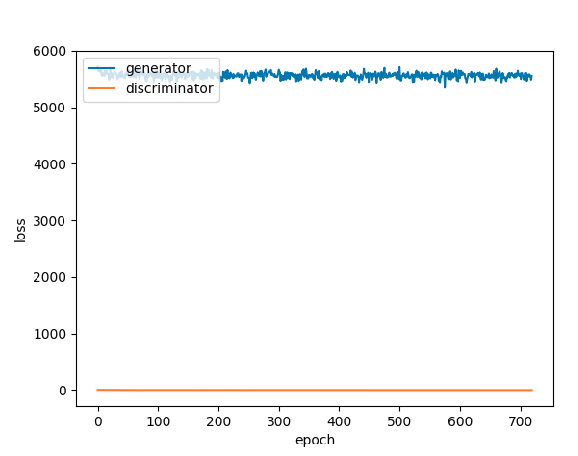
\includegraphics[width=9cm, height=8cm]{loss_Unit.png}
    \caption{\textit{Perte du générateur en bleu et celle du discriminateur en orange sur un peu plus de 700 époques}}
    \label{fig:perte_Unit}
\end{figure}


\vspace{5mm}

Pour répondre aux limites observées, j'ai essayé de moins entraîner le discriminateur par rapport au générateur, par exemple en ne l'entraînant qu'une époque sur 3. Cependant les résultats obtenus n'ont pas été meilleurs que ceux en figure 8 et visuellement, les productions du modèle sont peu fiables, voir figure 9. Ainsi, il est évident que le raffinage du modèle pour qu'il puisse être utilisé a joué un rôle dans cet échec. De plus, il est possible que sa complexité, rassemblant 3 modèles en 1 (VAE, coGAN et GAN) nuise à l'apprentissage. Enfin, il est possible que ce modèle soit inadapté pour le problème posé, car le modèle de Unit comme décrit n'est pas exactement le même que celui utilisé, pour des raison d'espace mémoire, et il ne peux donc pas apprendre la variabilité des données de cerveaux qui sont très variables et en trois dimensions. 

\vspace{5mm}
\begin{figure}[H]
\centering
\begin{subfigure}{.2\textwidth}
  
\includegraphics[width=2cm, height=4cm]{X1_150.png}
  \label{fig:sub1}
\end{subfigure}%
\begin{subfigure}{.2\textwidth}
  
\includegraphics[width=2cm, height=4cm]{fake_X2_150.png}
  \label{fig:sub2}
\end{subfigure}
\caption{\textit{Résultats de la transformation d'une image de squelette après 700 époques d'entraînement}}
\label{fig:res_Unit}
\end{figure}


\vspace{0.5cm}

\textbf{Vnet}\\

\vspace{1mm}

La complexité du Unit \cite{liu_unsupervised_2018} est sûrement la cause principale de mon échec à le rendre efficace pour le problème posé. Il semblait logique alors de se tourner vers un modèle déjà connu pour son efficacité dans le domaine médical comme vu dans l'état de l'art section III.3. Le modèle arrive rapidement à des résultats, même si quelques problèmes d'adaptation du modèle classique à notre sujet on été rencontrés au début.
Sur la figure \ref{fig:perte_vnet}, on remarque que la perte descend rapidement et converge vers 5 environ. Cela suggère que la transformation est plutôt fiable à nos attentes.

\vspace{5mm}
\begin{figure}[H]
    \centering
    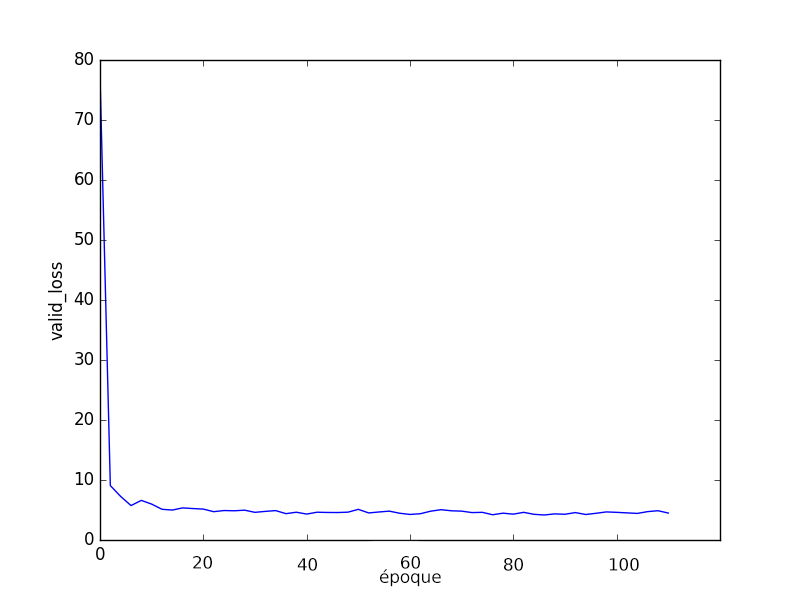
\includegraphics[width=9cm, height=8cm]{valid_loss_vnet.png}
    \caption{\textit{Perte de validation du Vnet après environ 110 époques }}
    \label{fig:perte_vnet}
\end{figure}

\vspace{5mm}

Après 20 époques, le modèle stagne et l'on arrive à une transformation proche de l'originale:


\vspace{5mm}

\begin{figure}[H]
\centering
\begin{subfigure}{.2\textwidth}
  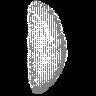
\includegraphics[width=4cm, height=4cm]{gw1_10.png}
  \label{fig:sub1}
\end{subfigure}%
\begin{subfigure}{.2\textwidth}
  
\includegraphics[width=4cm, height=4cm]{gw1_70.png}
  \label{fig:sub2}
\end{subfigure}
\begin{subfigure}{.2\textwidth}
  
\includegraphics[width=4cm, height=4cm]{gw4_130.png}
  \label{fig:sub2}
\end{subfigure}
\caption{\textit{Image générée par le Vnet après 10, 30 et 50 époques}}
\label{fig:res_Vnet}
\end{figure}


\vspace{5mm}

\begin{figure}[H]
\centering
\begin{subfigure}{.2\textwidth}
  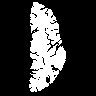
\includegraphics[width=4cm, height=4cm]{data4_130.png}
  \label{fig:sub1}
\end{subfigure}%
\begin{subfigure}{.2\textwidth}
  
\includegraphics[width=4cm, height=4cm]{target4_130.png}
  \label{fig:sub2}
\end{subfigure}
\caption{\textit{Images originales de squelette du sujet à gauche et même image mais en gris-blanc à droite}}
\label{fig:res_Unit2}
\end{figure}

\vspace{1cm}

On remarque figure \ref{fig:res_Vnet} que le modèle apprend progressivement à recréer des sillons de plus en plus précisément. Globalement, la \textit{Cross entropy} permet de favoriser la probabilité d'un voxel blanc à l'intérieur du cerveau, gris à l'extérieur et en arrière-plan du noir car le modèle ne se trompe pas sur des zones communes à tous les humains. On en conclut que le Vnet comprend la notion de substance blanche, intérieure au cortex, et y associe la notion de substance grise la recouvrant la surface du cerveau. Malgré cela, on observe que les sillons ne sont pas encore bien tracés. 

\vspace{5mm}

Le modèle doit donc davantage être entraîné pour finir par capturer ces éléments de manière plus détaillée. Je n'ai pas poursuivi le projet plus loin car j'avais déjà passé 2 mois de mon stage dessus, il constituait un entraînement et une manière de prendre en main les outils nécessaire aux traitement d'images cérébrales. Je me suis donc concentré sur mon projet principal sur les GANs. Néanmoins, je suis certain que ce modèle peut totalement convenir aux attentes, sûrement en le rendant plus profond et sur un nombre d'époques plus grand, ce qui lui permettrait un attention aux détails accrue.


\newpage

\subsection{Projet n°2 : Apprentissage de la variabilité corticale par les GANs}

Dans cette partie, l'objectif des réseaux implémentés est autre. On va travailler exclusivement avec des images de squelettes de cerveaux. Le but est de travailler sur plusieurs architectures de GANs afin d'apprendre une représentation des sillons humains. 
Nous avons décidé de complexifier légèrement ces modèles en ajoutant un encodeur à ces architectures. En effet, le générateur permet d'aller de l'espace latent vers l'espace des images, mais nous avons également besoin du processus inverse pour bien évaluer notre modèle et pour être capable de projeter nos images dans l'espace latent. Ainsi comme déjà fait dans l'article \textit{WGAN-based Autoencoder Training Over-the-air} publié en 2020 ou le f-AnoGAN en 2019, nous ajoutons un encodeur qui prend en entrée une image de squelette avant le générateur \cite{dorner_wgan-based_2020} \cite{schlegl_f-anogan_2019}. 


\subsubsection{GAN classique}
\vspace{5mm} 

Nous allons dans cette partie nous intéresser en profondeur aux différents types de \textit{Générative Adversarial Networks} \cite{goodfellow_generative_2014}. Comme expliqué dans l'état de l'art cf. section III.1, tous ces modèles reposent sur un système de compétition entre un générateur et un discriminateur. Le générateur, à partir d'un bruit de dimension fixe, crée des images de plus en plus réalistes dans le domaine choisi et le discriminateur doit s'améliorer pour pouvoir discerner les vraies images des images générées et donne une probabilité que l'image en entrée soit vraie.

Ces deux modules sont alors itérativement améliorés au fur et à mesure des époques d’entraînement via rétro-propagation. En effet, on définit une fonction d’erreur, ou \textit{loss}, qui détermine à quel point les différents modules ont appris à faire leurs tâches respectives:
 

\begin{equation}
    \min_{G} \max_{D}V(D,G)= \mathbb{E}_{x\sim p_{reel}(x)) }[logD(x)] + \mathbb{E}_{x\sim p_{z}(z)) }[log(1 - D(G(z))])
\end{equation}

\begin{figure}
    \centering
    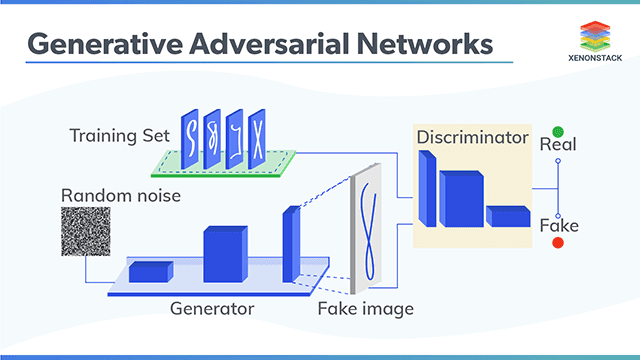
\includegraphics[width=11cm, height=7cm]{generative-adversarial-networks-applications-xenonstack.png}
    \caption{\textit{Schéma d'un GAN, image trouvée sur www.xenonstack.com}}
    \label{fig:GAN}
\end{figure}


Ici on ne définit qu'une seule fonction de perte pour les deux modules, où le générateur visera à la diminuer, lorsqu'au contraire, le discriminateur aura pour tâche de la maximiser.
 En effet, x dans cette formule représente une image de l'espace d'entrée et z un bruit.
 On a alors \textit{D(x) } la sortie du discriminateur lorsqu'on lui donne en entrée un image réelle, et \textit{D(G(z))} sa sortie lorsqu'on lui donne une image générée par le générateur. Plus la valeur du discriminateur est proche de 1, plus il considère que l'image est réelle, on comprend bien alors que pour celui-ci, il faut maximiser les deux termes.
Le premier terme est l'espérance du logarithme du discriminateur: lorsqu'il reçoit une image réelle, le disciminateur devrait sortir un scalaire proche de 1. Le deuxième terme est l'espérance de la sortie du discriminateur lorsque celui-ci reçoit une image du générateur. Le discriminateur doit donc apprendre à sortir une valeur proche de 0, et ainsi doit maximiser l'ensemble du deuxième terme. Le raisonnement est exactement inverse pour le générateur.

Ceci correspond au fonctionnement du GAN classique comme décrit par Ian Goodfellow dans son papier de 2014 \cite{goodfellow_generative_2014}.\\

Dans ce projet, il a été décidé d'ajouter un encodeur avant le générateur. En effet, il est très utile d'apprendre à un module en plus la correspondance entre une image et sa représentation latente. Cette fonction sera fortement utilisée lors de l'analyse de l'espace latent section V.2.6. On a alors un modèle de GAN revisité ci-dessous figure \ref{fig:Ganmodif}.

\vspace{1cm}
\begin{figure}[H]
    \centering
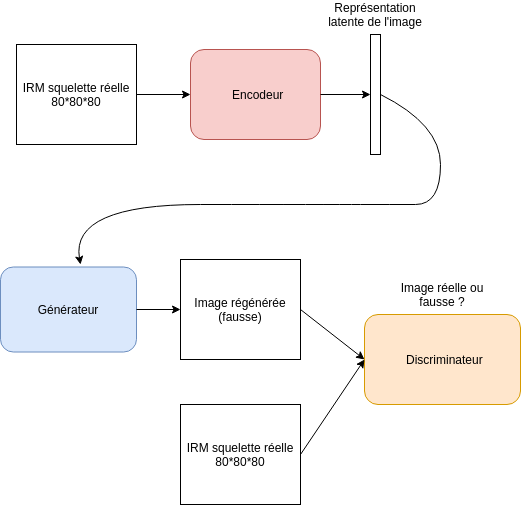
\includegraphics[width=11cm, height=10cm]{schemaGan.png}
    \caption{\textit{Schéma du GAN modifié }}
    \label{fig:Ganmodif}
\end{figure}

\vspace{1cm}

Le GAN classique comporte néanmoins quelques problèmes qui complexifient son utilisation. 
En effet, cette dualité dans le modèle, le double entraînement du générateur et du discriminateur sur une perte commune, perturbe l'entraînement, le rendant très instable. Il est ainsi compliqué pour le modèle de converger. 

De plus, le discriminateur peut être trop entraîné par rapport au générateur, on a alors un problème de disparition du gradient. En effet, le gradient alors très faible, tend vers 0 lors de la descente de gradient à travers les différentes couches du générateur et le discriminateur donne alors trop peu d'informations pour que le générateur s'améliore.

Enfin, le modèle peut tomber dans ce qu'on appelle le \textit{mode collapse.} En général, on veut que notre GAN puisse générer une grande variété d'images, qu'il capture la variabilité des images réelles et soit diversifié dans ses sorties. Cependant, si un générateur produit une sortie particulièrement plausible, il peut apprendre à ne produire que cette sortie. Le générateur essaie toujours de trouver la sortie qui semble la plus plausible au discriminateur. Si le générateur commence à produire la même sortie (ou un petit ensemble de sorties) encore et encore, la meilleure stratégie du discriminateur est d'apprendre à toujours rejeter cette sortie. Mais si la génération suivante du discriminateur reste coincée dans un minimum local et ne trouve pas la meilleure stratégie, il est alors trop facile pour l'itération suivante du générateur de trouver la sortie la plus plausible pour le discriminateur actuel. Chaque itération du générateur sur-optimise pour un discriminateur particulier, et le discriminateur ne parvient jamais à apprendre à sortir du minimum local. En conséquence, les générateurs tournent autour d'un petit ensemble de types de sortie. Cette forme d'échec du GAN est appelée \textit{mode collapse.} \\

Pour ces raisons, le GAN classique d'Ian Goodfellow est insuffisant et ne peut être utilisé pour des tâches complexes tel quel. Mais il a été la base d'une multitude d'autres réseaux ayant leurs propres spécificités et utilité, dont nous allons en voir quelques unes pour répondre au problème posé.

\subsubsection{Wasserstein GAN}

Le modèle classique du GAN, bien que novateur, est insuffisant pour arriver à des résultats satisfaisants pour des données avec un peu de variance. Une subtile nuance mais extrêmement efficace a été introduite en 2017 \cite{arjovsky_wasserstein_2017}. 
Au lieu de la définition de perte classique, on va utiliser une nouvelle métrique, la distance de Wasserstein. C'est le coût minimum de transport de la masse lors de la conversion de la distribution de données g (générée par le générateur) en distribution de données r (distribution réelle). \vspace{5mm} 

\centerline{\(W(\mathbb{P}_{r},\mathbb{P}_{g}) = \inf_{\gamma\in\Pi(\mathbb{P}_{r},\mathbb{P}_{g})}\mathbb{E}_{(x,y)\sim \gamma }[\left \| x-y \right \|] \)(3)} \\

\vspace{5mm} 

Avec cette nouvelle métrique, le gradient est plus lisse et apprend mieux même si le générateur ne produit pas de bonnes images. Cette définition peut s'écrire autrement grâce à la dualité de Kantorovich-Rubinstein, on obtient alors:\vspace{5mm} 

\centerline{\(W(\mathbb{P}_{r},\mathbb{P}_{\theta }) = \sup_{\left \| f \right \|_{L} \leq 1}\mathbb{E}_{x\sim \mathbb{P}_{r } }[f(x)] - \mathbb{E}_{x\sim \mathbb{P}_{\theta } }[f(x)]\) (4)}
\vspace{5mm}

Cette définition est plus pratique et permet une application immédiate aux GANs. Il reste néanmoins à bien définir les termes. En effet, f ici représente une fonction 1-\textit{Lipschitzienne}, c'est à dire qui vérifie pour tout  \(x_{1}\) et \(x_{2}\) dans son domaine de définition: \vspace{5mm} 

\centerline{\(\left | f(x_{1}) - f(x_{2}) \right |\leq \left |x_{1} - x_{2}\right |\) (5)}
\vspace{5mm}

Pour calculer la distance de \textit{Wasserstein}, il suffit donc de trouver une fonction 1-\textit{Lipschitzienne}. Comme tout autre problème d'apprentissage profond, nous pouvons construire un réseau profond pour l'apprendre. En effet, ce réseau est très similaire au discriminateur D, mais sans la fonction sigmoïde et il produit un score (non borné) plutôt qu'une probabilité. Ce score peut être interprété comme le degré de réalité des images d'entrée. Le discriminateur est rebaptisé "critique" pour refléter son nouveau rôle. 
Enfin, il faut imposer la contrainte de la 1-\textit{Lipschitzianité} du discriminateur. Pour ce faire on va effectuer un\textit{ gradient clipping},  c'est-à-dire que l'on introduit un hyperparamètre 'c' qui va restreindre les valeurs des poids du discriminateur, alors contraints de se situer entre [-c , c] (c est classiquement mit à 0.01).\\

Le wGAN répond aux problèmes de \textit{mode collapse} et de déséquilibre des modules dû à l'indépendance d'entraînement entre le générateur et le discriminateur. En effet, comme le discriminateur évalue la qualité de l'image plutôt que de sortir une probabilité, on n'a plus le problème de disparition du gradient quand le générateur est peu performant.

\subsubsection{Wasserstein GAN avec \textit{gradient penalty}}

Le wGAN est une grande avancée dans l'essor des GAN, néanmoins, en résolvant ses plus gros problèmes, d'autres limites apparaissent. Ce modèle est extrêmement sensible à l'hyperparamètre c qui se comporte comme une régulation des poids. Il réduit la capacité du modèle f et limite la possibilité de modéliser des fonctions complexes. Dans notre cas, il est nécessaire d'avoir un modèle qui puisse capturer une grande variété de motifs de sillons et avoir une architecture qui soit restreinte dans sa capacité d'apprentissage ne pourrait satisfaire à nos exigences. Il faut donc un autre moyen d'imposer la 1-\textit{Lipschitzianité} du discriminateur, ou critique. 

\vspace{5mm} 

Le dernier modèle implémenté est donc le Wasserstein GAN avec pénalité sur le gradient \cite{gulrajani_improved_2017}. La formule (5) peut aussi être interprétée comme le fait qu'une fonction 1-\textit{Lipschitzienne} doit avoir des gradients au maximum égaux à 1.
Au lieu d'appliquer un \textit{gradient clipping}, le wGAN-GP pénalise le modèle si la norme du gradient s'éloigne de sa valeur cible qui est donc 1. On remarque dans la formule (6) ci-dessous qu'il y a un terme \(\lambda\) devant le \textit{gradient penalty} qui pondère ce dernier terme, classiquement mis à 10.

\vspace{2mm}

\centerline{\(L = \mathbb{E}_{\tilde{x}\sim\mathbb{P}_{g} }[D(\tilde{x})] - \mathbb{E}_{x\sim\mathbb{P}_{r} }[D(x)] + \lambda\mathbb{E}_{\tilde{x}\sim\mathbb{P}_{\tilde{x}} }[(\left \| \nabla_{\tilde{x}}D(\hat{x}) \right \|_{2}-1)^{2}]\)} (6)}


\subsubsection{Résultats}

\textbf{GAN}\\

\vspace{1mm}


Comme pour le projet précédent, j’implémente une normalisation de type\textit{ minimum distance} pour les images de squelettes. afin de discrétiser les valeurs prises par ceux-ci. Cependant, au lieu de binariser ceux-ci, on impose une \textit{cross-entropy }sur 3 valeurs:
\begin{itemize}
\item  0 : Pixel dans le cerveau
\item 11 : Pixel hors du cerveau
\item 60 : Pixel dans un sillon 
\end{itemize}
 
Ensuite, on reprend classiquement l'architecture du GAN comme dans son article fondateur \cite{goodfellow_generative_2014} en y accolant un encodeur juste avant le générateur. Sur la figure \ref{fig:Ganmodif} un schéma du GAN modifié que j'utilise. Toutes les couches sont denses (\textit{fully connected}) pour le générateur et le discriminateur. \\


Pour l'apprentissage, on utilise la définition de perte classique du GAN (2), et la perte de reconstruction L2 pour l'encodeur. Cette perte est celle des moindres carrés pixel par pixel. Elle permet donc d'évaluer l'apprentissage du modèle mais surtout sa capacité à comprendre les données. En effet avec l'encodeur, on fait correspondre une image avec un point dans l'espace latent qui aura beaucoup moins de dimensions que l'espace image de base (de \(80^{3}\) à 1024). Ce code est ensuite donné au générateur qui recrée l'image de squelette aux dimensions initiales. Durant le processus, il y a une perte d'information pixel par pixel lors de la compression de l'image par l'encodeur. On force donc au modèle d'apprendre les différents motifs des sillons.\\

Grâce à l'expérience acquise lors du projet n°1, l'adaptation du GAN à notre problème a été plutôt rapide, cependant les résultats se sont avérés peu performants. Comme vu précédemment dans la section V.2.1 sur le GAN, l'entraînement est très instable et peine à apprendre comme on peut le voir figure \ref{fig:perte_GAN}.

\begin{figure}[H]
    \centering
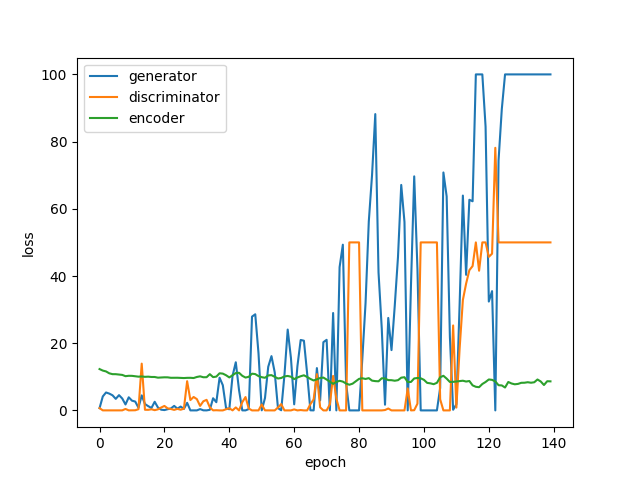
\includegraphics[width=10cm, height=9cm]{gan3.png}
    \caption{\textit{Courbes de pertes des différents modules du GAN}}
    \label{fig:perte_GAN}
\end{figure}

Sur la figure \ref{fig:perte_GAN}, on observe que les performances du générateur et du discriminateur alternent indéfiniment alors que l'encodeur apprend très lentement, sûrement perturbé par l'instabilité des autres modules. Le modèle atteint vite ses limites, environ après 100 époques d'entraînement et la reconstruction est peu fiable comme on peut le voir figure \ref{fig:reco_GAN}. Le GAN apprend la forme du cerveau et sa position ainsi que l'arrière-plan sans arriver à reconstruire les sillons.

\begin{figure}[H]
\centering
\begin{subfigure}{.2\textwidth}
    
\includegraphics[width=4cm, height=4cm]{data1_40.png}
  \label{fig:sub1}
\end{subfigure}%
\begin{subfigure}{.2\textwidth}
  
\includegraphics[width=4cm, height=4cm]{target1_40.png}
  \label{fig:sub2}
\end{subfigure}
\caption{\textit{Reconstruction du GAN}}
\label{fig:reco_GAN}
\end{figure}

Le dc-GAN a également été implémenté mais les résultats n'étant pas satisfaisants, ils ne sont pas décrits.
\vspace{0.5cm}

\textbf{wGAN}\\

Il est temps de passer au wGAN pour essayer de stabiliser l'entraînement en espérant obtenir de meilleurs résultats. L'architecture reste sensiblement la même à la différence que j'essaye d'optimiser au maximum l'architecture, toujours sous la contrainte de la mémoire GPU disponible sur serveur distant. J'augmente notamment le nombre de couches dans l'encodeur et le générateur, mais contrairement au GAN classique, ces modules comportent uniquement des couches convolutives. Ensuite comme expliqué section V.2.2, je transforme le discriminateur en critique. Il a donc maintenant pour rôle de la régression linéaire plutôt que de la classification comme dans le GAN. Enfin, la définition de la perte est adaptée.
On obtient alors une évolution de la perte décrit dans figure \ref{fig:perte_wGAN}.

\begin{figure}[H]
    \centering
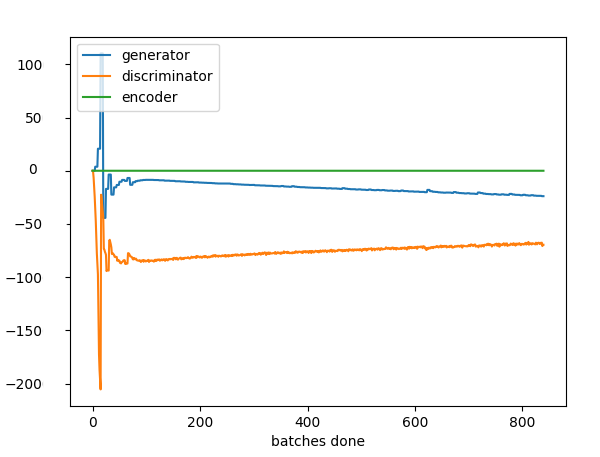
\includegraphics[width=10cm, height=9cm]{wgan.png}
    \caption{\textit{Courbes de pertes des différents modules pour le wGAN}}
    \label{fig:perte_wGAN}
\end{figure}

On voit que la perte du discriminateur prend des valeurs démesurément grandes puis diminue lentement. Celle du générateur continue à diminuer tandis que l'encodeur peine à apprendre.Le discriminateur est en réelle difficulté à évaluer les images de squelette, ce qui fait diminuer la perte du générateur sans pour autant améliorer la qualité des images générées, comme l'atteste la constance de la perte de l'encodeur. Visuellement, on obtient des images globalement en forme de cerveaux mais sans sillons, comme on peut le voir dans la figure \ref{fig:res_wGAN} ci-dessous.

\begin{figure}[H]
    \centering

\includegraphics[width=4cm, height=4cm]{target1_60.png}
    \caption{\textit{Image reconstruite du wGAN}}
    \label{fig:res_wGAN}
\end{figure}

Cela peut s'expliquer par la forte contrainte imposée au discriminateur et mentionnée section V.2.2. Les motifs cérébraux sont toujours trop complexes pour cette architecture. 
Pour essayer de résoudre ce problème, les différentes classes de voxels ont été pondérées lors du calcul de la perte. Comme le réseau peine à reconstruire les sillons et qu'ils constituent l'objet principal de l'étude, il semble logique de porter plus d'importance à ceux-ci. Ainsi, j'ai itérativement essayé de pondérer la \textit{cross-entropy} pour favoriser l'apprentissage des sillons. J'ai alors gardé les deux autres classes à une valeur de 1 et 5 comme pondération pour les sillons. Cette méthode n'a pas permis d'apporter de bons résultats comme on peut l'observer sur la figure \ref{fig:res_wGAN2}. En effet, le réseau se contente d'épaissir le contour du cerveau pour optimiser sa perte. Cela n'a donc pas réussi à favoriser un meilleur apprentissage. Néanmoins, cette pondération a été conservée pour la suite du travail car elle est pertinente pour ce projet.

\begin{figure}[H]
    \centering

\includegraphics[width=4cm, height=4cm]{target4_180.png}
    \caption{\textit{Image reconstruite du wGAN après pondération}}
    \label{fig:res_wGAN2}
\end{figure}

\textbf{Wgan-gp}\\

Afin de faciliter la tâche d'apprentissage, nous avons décidé de ne plus travailler sur des hémisphères mais plutôt sur des\textit{ crops}, c'est-à-dire des zones spécifiques du cerveau. La région d'intérêt étant plus petite, elle comprend moins de sillons et donc moins de variabilité. Notre étude se focalise dès lors sur la région des branches terminales du sillon temporal supérieur (S.T.s), région extrêmement variable entre les individus et qui pourrait être liée à des troubles de l'autisme. Après avoir adapté le pré-traitement en conséquence, j'ai adapté le modèle avec ces nouvelles entrées. Il faut ensuite ajouter le terme de pénalité de la norme et enlever le \textit{clipping }des gradients.

Le choix des hyperparamètres a d'abord été empirique, par essai et erreur puis globalement confirmé par un \textit{grid search}, c'est-à-dire que le modèle a été testé pour une échelle de valeur donnée sur quelques paramètres par session de recherche. Un extrait d'une session de \textit{grid search }est en figure \ref{fig:grid}.

\begin{figure}[H]
    \centering
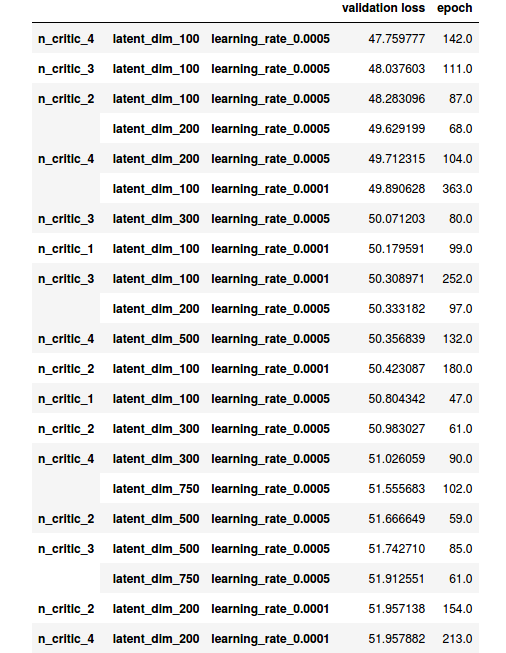
\includegraphics[width=7.5cm, height=8cm]{grid.png}
    \caption{\textit{Grid search sur 3 hyperparamètres : le pas d'apprentissage, taille de l'espace latent et cadence d'entraînement du discriminateur}}
    \label{fig:grid}
\end{figure}

De même que les autres modèles, l'architecture du wGAN-gp que j'ai utilisé est décrit en détail dans les annexes 4, 5, 6 et 7. En structure globale il ne diffère pas beaucoup des autres GANs, il se distingue par son terme en plus dans la définition de la perte correspondant à la pénalité du gradient du discriminateur, mais aussi par le nombre de couches utilisées. En effet, ce modèle est beaucoup moins "lourd" que les autres et, grâce à son efficacité, j'ai pu réduire le nombre de couches afin de fluidifier l'entraînement. Ce modèle m'a demandé beaucoup de travail d'optimisation, toujours sous les contraintes de la mémoire. On arrive avec un espace latent de 1728 dimensions, un peu plus que sur les précédents modèles. 

Sur la figure \ref{fig:loss_gp}, on remarque que les courbes de perte du générateur et discriminateur sont très épaisses, ce qui veut dire qu'ils fluctuent fortement jusqu'à environ 175 époques où ils se stabilisent. Le générateur apprend beaucoup mieux qu'avec les autres modèles et tient le discriminateur en échec pendant tout l'entraînement, ce qui ne veut pas dire que celui-ci n'apprend pas. De son côté, l'encodeur apprend de manière assez linéaire et converge vers une perte de 5 environ.

\begin{figure}[H]
    \centering
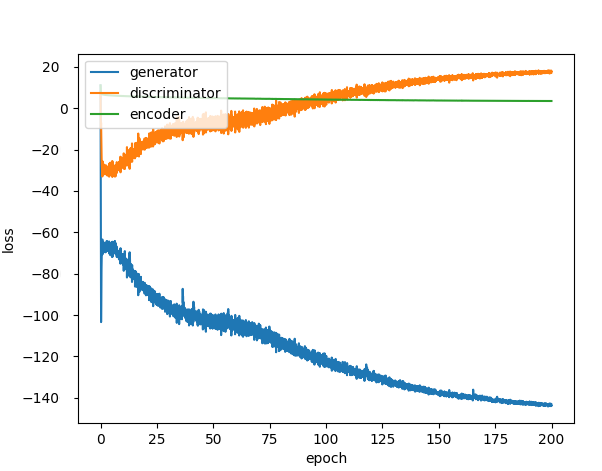
\includegraphics[width=8cm, height=8cm]{lossgangp.png}
    \caption{\textit{Graphique de perte des modules du wGAN-gp}}
    \label{fig:loss_gp}
\end{figure}

Visuellement, on remarque que les reconstructions sont de plus en plus fiables aux originaux, avec des bordures de plus en plus précises pour les sillons. Ci-dessous, la figure \ref{fig:reco_GANgp} représente les résultats des reconstructions sur une image de l'ensemble de validation durant l'entraînement.

\begin{figure}[H]
\centering
\begin{subfigure}{.2\textwidth}
    
\includegraphics[width=4cm, height=4cm]{valid_target199_2.png}
  \label{fig:sub1}
\end{subfigure}%
\begin{subfigure}{.2\textwidth}
  
\includegraphics[width=4cm, height=4cm]{valid_img199_2.png}
  \label{fig:sub2}
\end{subfigure}
\caption{\textit{Reconstruction du wGAN-gp sur une image de validation à droite et image originale à gauche}}
\label{fig:reco_GANgp}
\end{figure}

Ce modèle est le plus abouti des modèles que j'ai créés. La reconstruction est presque parfaite, avec une épaisseur des sillons double par rapport aux images originales néanmoins.


\subsubsection{Test du meilleur modèle}

Un modèle satisfaisant ayant été trouvé, il faut maintenant vérifier qu'il puisse être utile. En effet, il faut déjà être sûr qu'il n'est pas en surapprentissage, c'est-à-dire qu'il n'apprend pas à reconstruire par coeur les images d'entraînement. Pour ce problème, cela semble assez improbable car l'ensemble d'entraînement est constitué de 800 sujets environ et le réseau n'est pas assez profond. Pour vérifier cela, il suffit de tester le modèle sur des images jamais vues par le réseau. Au préalable, j'avais donc séparé les sujets du HCP (environ 1100) en trois ensembles, environ 800 pour l'entraînement, 200 pour la validation et 100 pour le test. C'est donc l'ensemble de validation que j'utilise pour affirmer que mon modèle n'est pas en surapprentissage et l'on peut voir figure \ref{fig:reco_GANgp} que la reconstruction est d'aussi bonne qualité pour l'ensemble de test que pour l'ensemble de validation.

\subsubsection{Analyse de l'espace latent}

Afin d'évaluer ce que le modèle a appris et la façon dont il a modélisé les sillons, nous avons exploré l'espace latent. Pour ce faire et pour chaque sections qui va suivre, il s'agit d'encoder les images de squelettes. On va donc à l'aide de plusieurs techniques comprendre comment il est constitué et évaluer sa qualité dans le contexte de détection d'anomalies.\\

\textbf{Interpolation entre deux cerveaux}

Tout d'abord, je voulais évaluer la continuité de cet espace. Pour cela, j'ai interpolé "en ligne droite" entre la représentation latente de deux squelettes de cerveaux au hasard dans le HCP. C'est-à-dire que j'ai pris l'encodage de deux images, et ai généré des images avec les codes intermédiaires entre les deux.  La figure \ref{fig:expl1} ci-dessous explique la méthodologie employée. On fixe le nombre de points intermédiaires voulu et pour chaque point on a son code dans l'espace latent égal à : \(u + \frac{k}{n} * (v-u) \), avec n le nombre de points voulu, u et v les deux codes des cerveaux à l'extrémité.

\begin{figure}[H]
    \centering
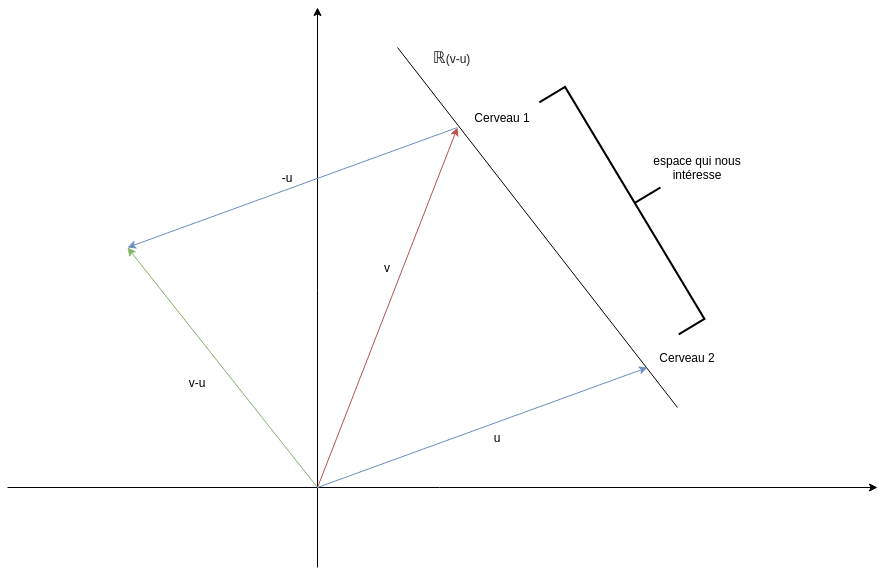
\includegraphics[width=13cm, height=8cm]{expl_ligne.png}
    \caption{\textit{Méthode d'interpolation dans l'espace latent}}
    \label{fig:expl1}
\end{figure}

On obtient alors les images présentées sur la figure \ref{fig:gen_inter}. Les images des deux squelettes originaux sont aux extrémités en haut à gauche et en bas à droite, entre les deux sont présentés les résultats des interpolations générées par le générateur. Les images de squelettes évoluent lentement d'un cerveau vers l'autre, les sillons changeant de manière plus au moins continue selon le choix du nombre d'échantillons.


\centerline{
\includegraphics[width=2cm, height=2cm]{fake_img.png}\hspace{5mm}
\includegraphics[width=2cm, height=2cm]{fake_img0.png}\hspace{5mm}
\includegraphics[width=2cm, height=2cm]{fake_img51.png}}
\centerline{
\includegraphics[width=2cm, height=2cm]{fake_img81.png}\hspace{5mm}
\includegraphics[width=2cm, height=2cm]{fake_img99.png}\hspace{5mm}
\includegraphics[width=2cm, height=2cm]{fake_img100.png}}
\begin{figure}[H]
    \centering
    \caption{\textit{Génération des cerveaux intermédiaires}}
    \label{fig:gen_inter}
\end{figure}

\textbf{Évaluation du \textit{clustering}}\\


On en conclut qu'on a alors un espace latent assez régulier, l'intérêt maintenant est d'étudier comment sont regroupés les différents sujets. Idéalement, on voudrait que le réseau crée plusieurs \textit{clusters}, regroupant les individus par caractéristiques corticales communes ce qui permettrait de caractériser et catégoriser les individus en termes de sillons. On va alors essayer de calculer un score de \textit{clustering}, il faut au préalable que l'on attribue à chaque point un groupe, et il faut ainsi fixer aussi le nombre total de groupes. On applique alors un algorithme de \textit{clustering} de type k-moyenne aux représentations latentes de l'ensemble de test afin d'en labéliser chaque point avec un \textit{cluster}. On va appliquer les k-moyennes avec différents nombres de \textit{cluster}, 2, 3, 4 et enfin 5 puis calculer le score silhouette pour chaque point.\\ 

Ensuite, pour évaluer la capacité du modèle à regrouper les données en un ou plusieurs groupes, j'ai utilisé le score Silhouette. Pour chaque point, son coefficient de silhouette est la différence entre la distance moyenne avec les points du même groupe que lui (cohésion) et la distance moyenne avec les points des autres groupes voisins (séparation). Si cette différence est négative, le point est en moyenne plus proche du groupe voisin que du sien : il est donc mal classé. À l'inverse, si cette différence est positive, le point est en moyenne plus proche de son groupe que du groupe voisin : il est donc bien classé.
On obtient alors les scores figure \ref{fig:expl2} ci dessous.

\begin{figure}[H]
    \centering
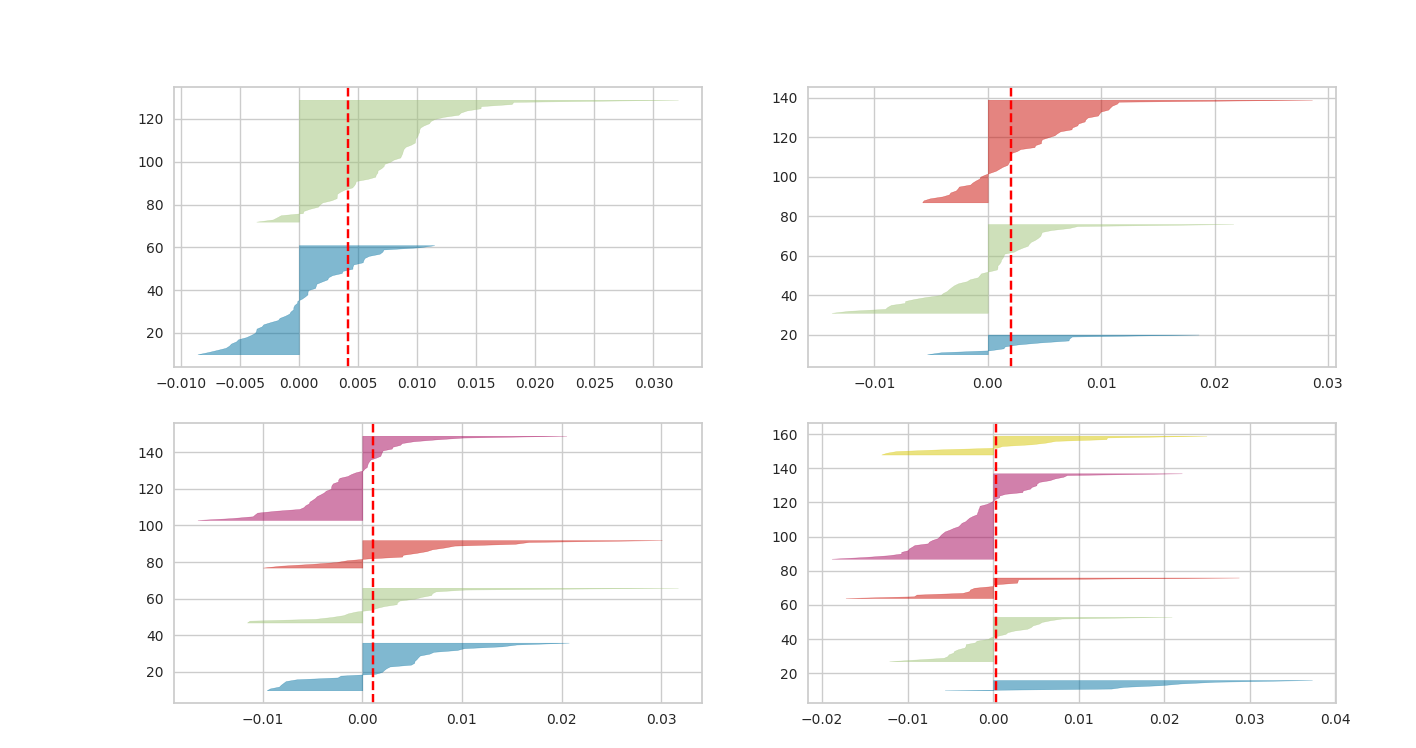
\includegraphics[width=12cm, height=8cm]{silhouettescore.png}
    \caption{\textit{Score Silhouette sur l'ensemble test avec 2,3,4 et 5 clusters}}
    \label{fig:expl2}
\end{figure}

Le graphique en haut à gauche correspond au score silhouette pour 2 \textit{clusters,} celui juste à droite pour 3 et ainsi de suite. Chaque ligne représente un cerveaux encodé et son score silhouette en abscisse.
En pointillés rouges est le score silhouette moyen pour chaque nombre de \textit{clusters} choisi. On remarque que, déjà pour 2 \textit{clusters} il est très faible, mais qu'il ne fait que diminuer en augmentant le nombre de \textit{clusters}.
Deux hypothèses peuvent être envisagées : Soit les cerveaux sont répartis de manière hasardeuse dans l'espace latent, soit, comme le laissait supposer l'étude d'interpolation précédente, il n'existe qu'une concentration de cerveaux, donc un seul \textit{cluster } où sont regroupés les squelettes de cerveaux.\\

\textbf{t-SNE}\\


Pour étudier la répartition des sujets dans l'espace latent et voir s'il existe un certain ordre, l'algorithme t-SNE (\textit{t-distributed stochastic neighbor embedding}) a été utilisé. C'est une technique de réduction de dimensions pour la visualisation de données qui permet de représenter un ensemble de points d'un espace à grande dimension dans un espace de deux ou trois dimensions. Les données peuvent ensuite être visualisées avec un nuage de points. L'algorithme t-SNE tente de trouver une configuration optimale selon un critère de théorie de l'information pour respecter les proximités entre points : deux points qui sont proches dans l'espace d'origine devront être proches dans l'espace de faible dimension. Toujours sur l'ensemble de test, j'ai alors appliqué l'algorithme, et on obtient la figure \ref{fig:tsne} ci-dessous.

\begin{figure}[H]
    \centering
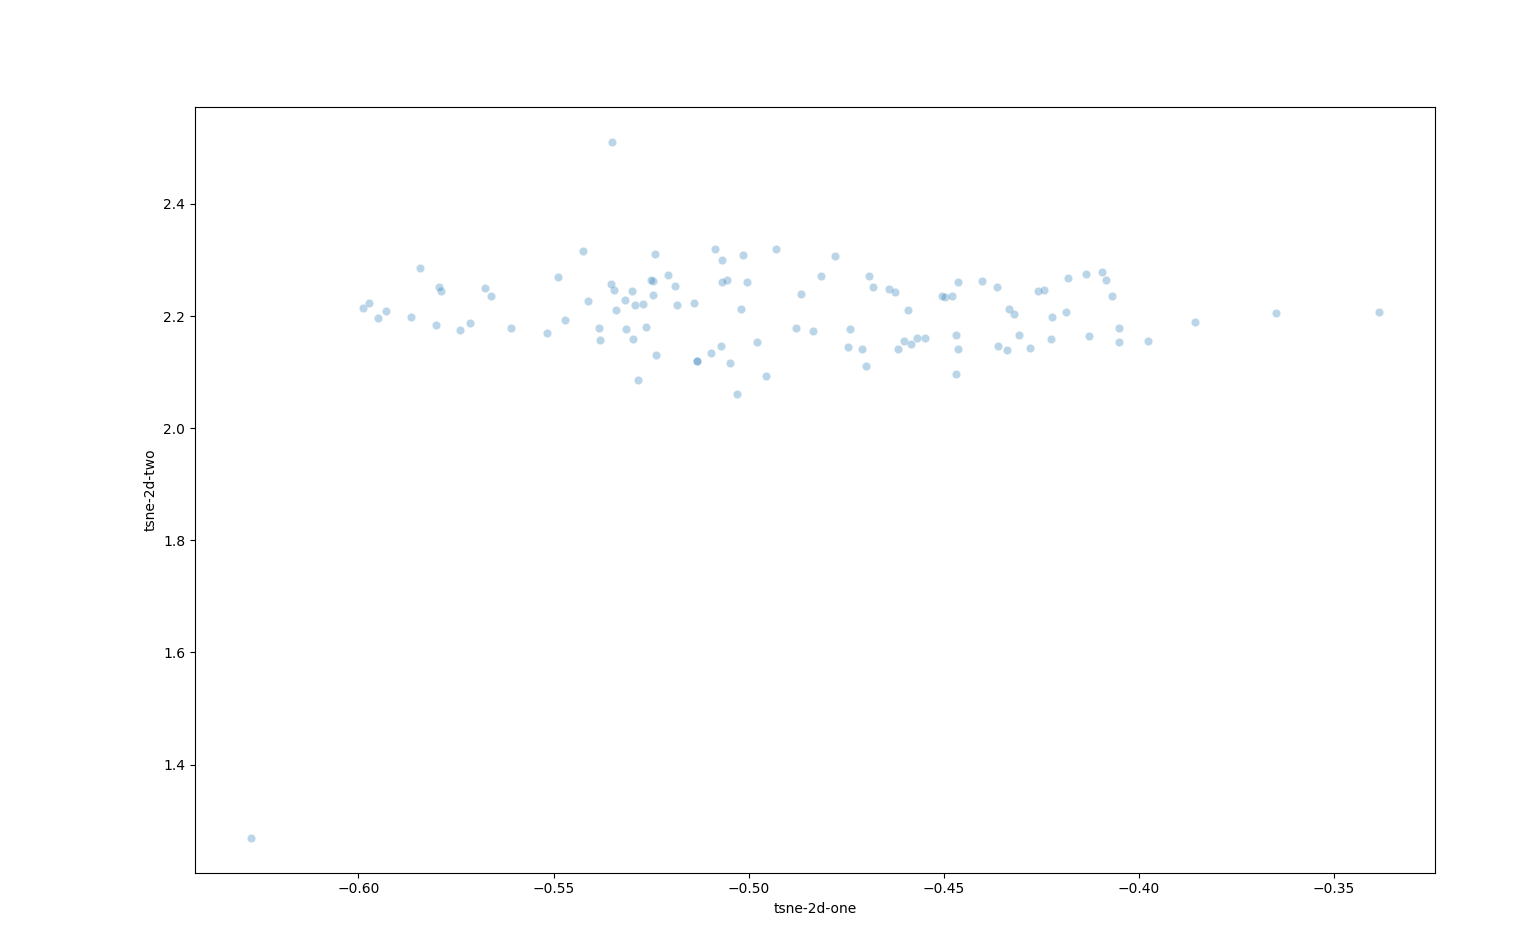
\includegraphics[width=13cm, height=7cm]{tsne.png}
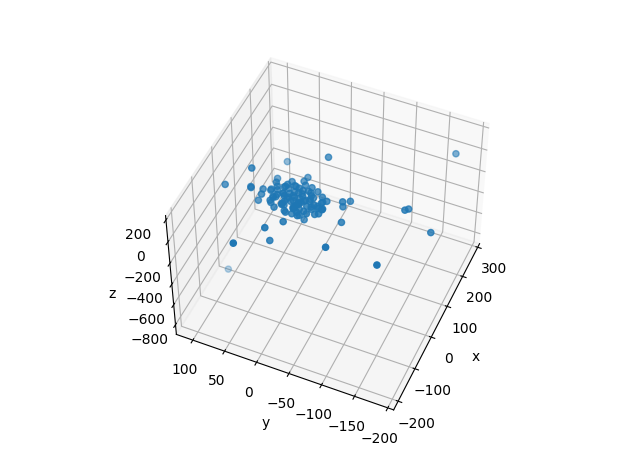
\includegraphics[width=10cm, height=7cm]{tsne3Dtest.png}
    \caption{\textit{Résultats du t-SNE en 2D et 3D sur l'ensemble de test encodé}}
    \label{fig:tsne}
\end{figure}

On observe que les cerveaux sont bien regroupés en un et un seul groupe. Ce résultat est encourageant dans la mesure où le but est de contribuer à une plus large étude de détection d'anomalies cérébrales. 

\vspace{1mm}

\textbf{Cerveau moyen}

\vspace{1mm}

Nous avons ici un réseau qui encode de manière proche les squelettes des cerveaux sains qu'on lui donne en entrée. On peut donc se demander à quel point il a appris cette notion de cerveau sain. L'expérience suivante consiste à chercher l'emplacement du centre de ce cluster et d'en générer l'image afin d'obtenir le "cerveau moyen". Pour cela, j'encode à nouveau tous les cerveaux de l'ensemble de test, je calcule la moyenne pour chaque dimension latente (1728) et je donne ce vecteur moyen au générateur. Je visualise le cerveau moyen généré en 3D grâce au logiciel de visualisation de cerveaux Anatomist de BrainVisa et figure \ref{fig:cerv_centre} images de ce cerveau.

\vspace{0.5cm} 

\centerline{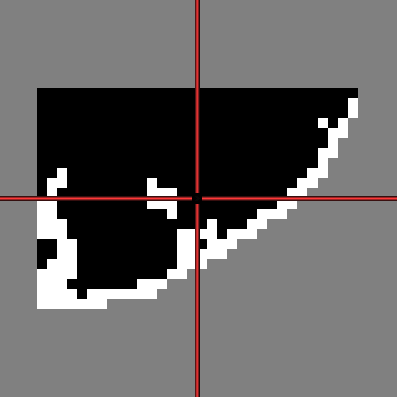
\includegraphics[width=4cm, height=4cm]{cervmoy1.png}\hspace{5mm}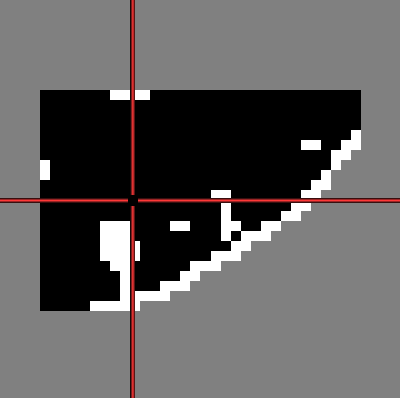
\includegraphics[width=4cm, height=4cm]{cervmoy12.png}\hspace{5mm}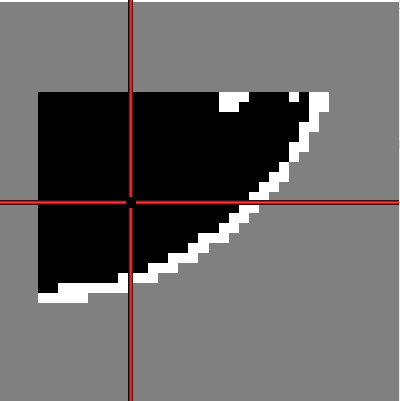
\includegraphics[width=4cm, height=4cm]{cervmoy13.png}}
\begin{figure}[H]
    \centering
    \caption{\textit{Quelques images du cerveau central}}
    \label{fig:cerv_centre}
\end{figure}

Il est très difficile d'identifier et nommer des éventuels sillons dans ce cerveau moyen. On peut toutefois remarquer qu'il ressemble fortement à un cerveau humain, en tout cas dans sa structure à défaut de comporter exactement tous les sillons.\\

\vspace{1mm}

\textbf{Étude avec \textit{Benchmarks}}\\

\vspace{1mm}

Enfin, une dernière méthode beaucoup plus qualitative pour évaluer le modèle est de lui donner des cerveaux comportant une anomalie. En effet, j'ai constitué plusieurs ensembles de squelettes de cerveaux.
Dans chaque cerveau de chaque ensemble, on enlève un sillon au hasard. La différence entre les ensembles est la taille (en voxels) du sillon supprimé. Ce paramètre nous l'appellerons bbox\_max et les valeurs choisies pour ce paramètre sont {0 (sujets normaux), 200, 500 et 800}.
Ci dessous, figure \ref{fig:bench} représente deux exemples de squelettes de cerveaux dont on a enlevé un sillon au hasard de taille différente.

\vspace{0.5cm} 

\centerline{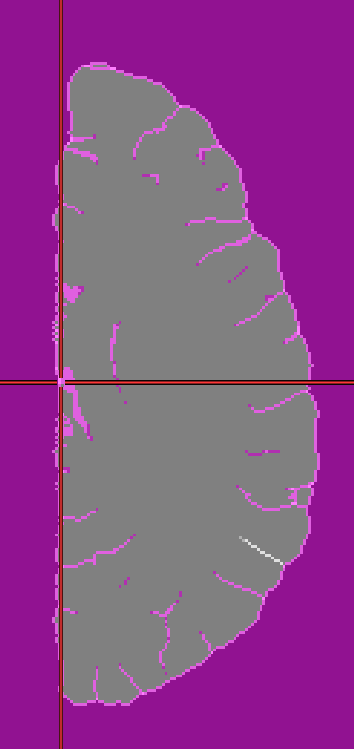
\includegraphics[width=3cm,height=6cm]{benchmark1.png}\hspace{5mm}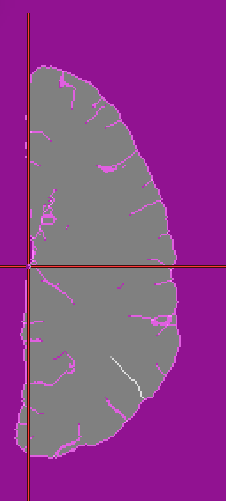
\includegraphics[width=3cm, height=6cm]{benchmark2.png}}
\begin{figure}[H]
    \centering
    \caption{\textit{Squelettes de cerveaux dont 1 sillon a été supprimé. Le sillon supprimé est représenté en blanc}}
    \label{fig:bench}
\end{figure}

Ici, les deux sillons supprimés que l'on peut voir en blanc sont le sillon temporal supérieur terminal ascendant antérieur gauche, à gauche, et le sillon temporal supérieur terminal ascendant postérieur gauche pour l'image de droite. Pour obtenir ces images j'ai superposé les cerveaux modifiés avec leurs images normale en blanc. \\

Maintenant, il ne reste plus qu'a visualiser la représentations de tous ces ensembles modifiés dans l'espace latent grâce l'algorithme t-SNE, figure \ref{fig:tsne2} ci-dessous. Tous les cerveaux sont labélisés avec leur valeur bbox\_max.

\begin{figure}
\centering
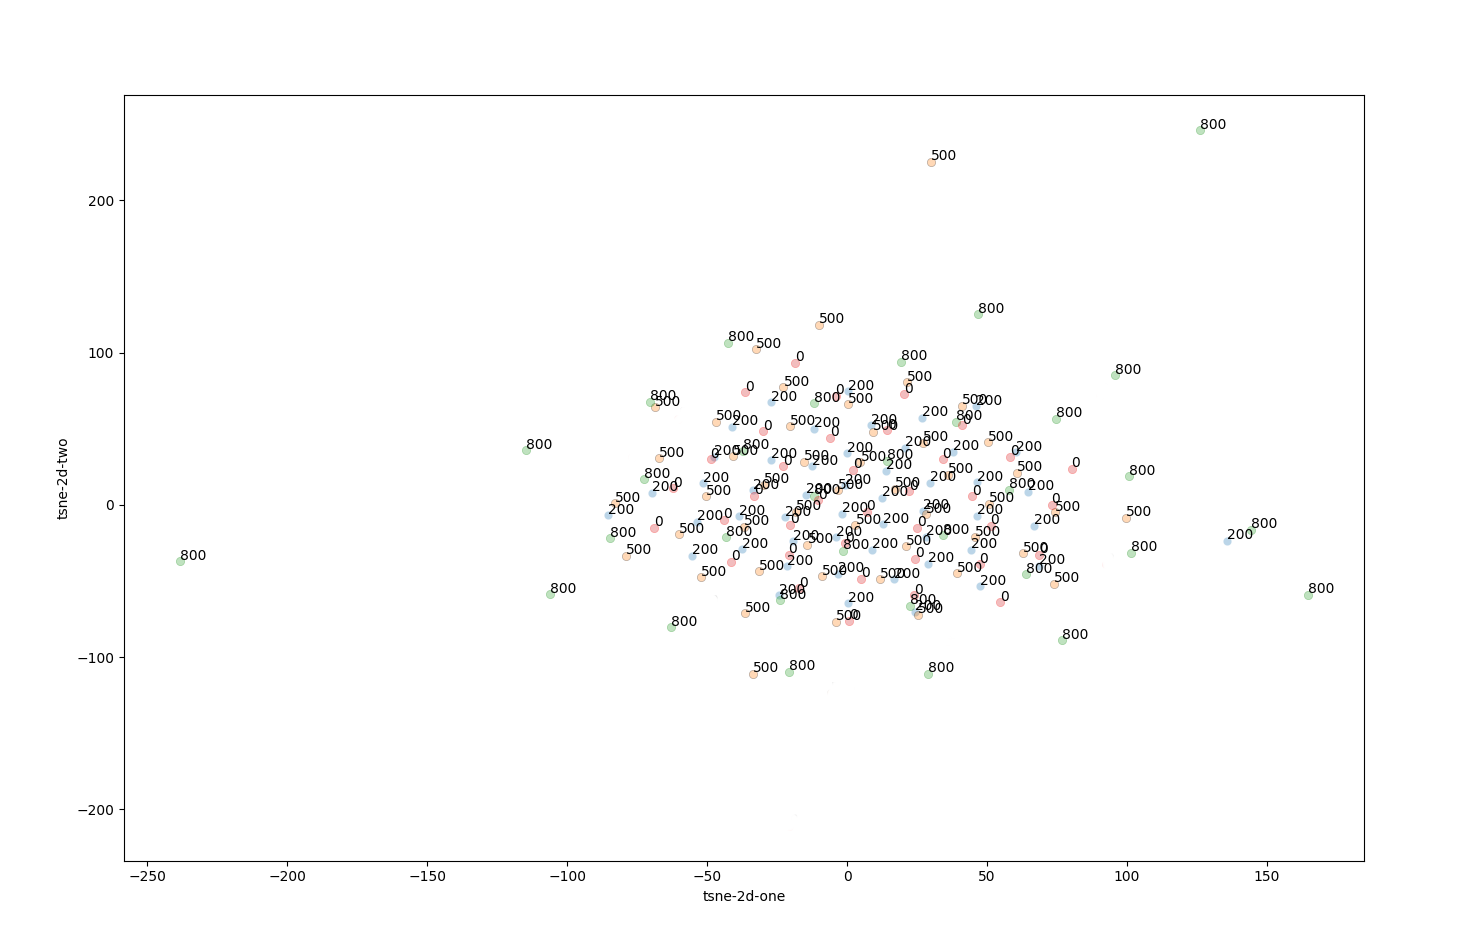
\includegraphics[width=15cm,height=9cm]{tsne_50b.png}
    \caption{\textit{T-SNE sur 3 ensembles de benchmark et un ensemble de test}}
    \label{fig:tsne2}
\end{figure}


Plus la valeur de bbox\_max est grande, plus il est susceptible que le sillon supprimé soit grand, et donc que le cerveau résultant soit différent d'un cerveau normal. On remarque alors que globalement pour des valeurs de bbox\_max faibles (200 et 500), les squelettes de cerveaux sont proches du cluster des cerveaux normaux, même en bordure de ceux-ci. En revanche, les cerveaux labélisés avec un bbox\_max de 800 sont à la périphérie de ce regroupement. Ainsi, il semblerait que  le modèle adapté du wGAN-gp peut, dans la majorité des cas, différencier une image de squelette de cerveau humain normale avec une image altérée sur cette partie du sillon temporal supérieur, très variable chez les humains.\\

\vspace{1cm}
\subsubsection{Limites du modèle}


Dans cette dernière partie, nous allons voir que ce modèle est encore loin d'être parfait.
Pour aller plus loin dans l'analyse de celui-ci, j'ai regardé ce que les dimensions dans l'espace latent codaient exactement. Contrairement à des modèles plus classiques comme un \textit{multi layer perceptron}, on s'attendrait à ce qu'un GAN bien entraîné, bien qu'on ne l'aie pas conditionné comme un cGAN ou infoGAN, ait appris des caractéristiques précises en lien avec la variabilité corticale humaine. Pour vérifier cela, j'ai tout d'abord établi un classement automatique de mes dimensions étant donné que mon espace latent est grand (1728 dimensions). La métrique utilisée est la suivante: Pour chaque dimension, on va encoder les cerveaux de l'ensemble de test. Puis, ce code va être légèrement modifié uniquement selon la dimension choisie et on va ensuite calculer la perte de reconstruction avec le modèle déjà entraîné sur le vrai code non-modifié, puis sur les codes modifiés. Le score est alors la différence entre la perte de reconstruction avec l'encodage normal et la perte en modifiant légèrement selon la dimension. En faisant la moyenne de ces scores pour chaque cerveau de l'ensemble, puis en itérant sur chaque dimension, on obtient alors un score pour chaque dimension de l'espace latent. Le but de cette métrique est de regarder à quel point chaque dimension est importante lors de la reconstruction d'une image de squelette. Plus le score est élevé, plus l'erreur de reconstruction a changé en modifiant selon cette dimension, donc plus elle est importante. Les résultats de ce classement sont présentés figure \ref{fig:range} ci-dessous. J'obtiens alors un top 20 de mes dimensions. On est alors sensé avoir déterminé quelles dimensions sont les plus significative pour le modèle, et le but maintenant et d'en découvrir la sémantique.

\begin{figure}[H]
\centering
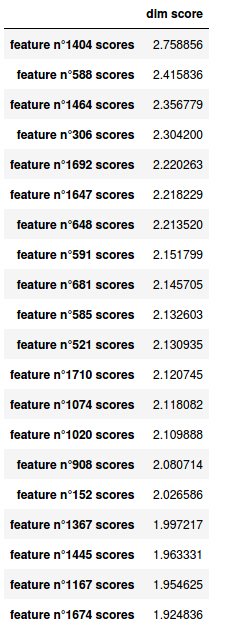
\includegraphics[width=4cm, height=10cm]{feature_score.png}
    \caption{\textit{Classement des 20 meilleures dimensions}}
    \label{fig:range}
\end{figure}

Une dernière étape est de déterminer comment les explorer de manière pertinente. L'idée est de partir d'une représentation latente d'un cerveau au hasard, puis de le faire varier selon la dimension voulue. Pour définir les bornes de cette exploration, on choisit les valeurs minimales et maximales des encodages de cerveaux pour chaque dimension. Ainsi, on peut donc explorer les dimensions du top 20 tout en restant dans le cluster des cerveaux sains. Les résultats obtenus pour le top 3 sont présentés figure \ref{fig:range2}.

\vspace{1cm}
\begin{figure}[H]
\centering
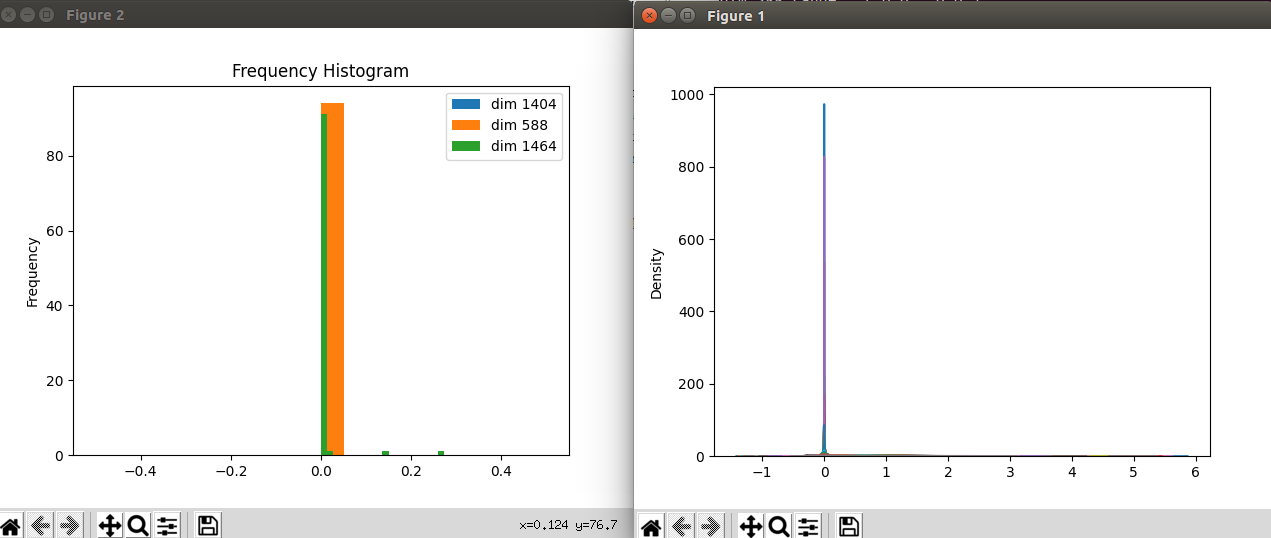
\includegraphics[width=13cm, height=6cm]{histotop3.png}
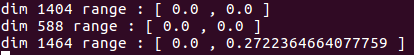
\includegraphics[width=5cm, height=0.8cm]{rangetop3.png}
    \caption{\textit{Extremums, histogrammes et courbes de densité pour les 3 meilleures dimensions}}
    \label{fig:range2}
\end{figure}

On remarque donc que pour les deux "meilleures" dimensions, l'encodage donne toujours 0. Il semble donc qu'une bonne partie des dimensions de l'espace latent ne code rien, et donc qu'il aurait fallu mieux choisir la dimension de l'espace latent en la diminuant. Lors de la conception de mon modèle, j'ai néanmoins été très contraint par la mémoire et les manières que j'ai trouvées pour pouvoir changer ce paramètre de dimension d'espace latent ont affaibli le modèle.

Néanmoins, on remarque sur la figure \ref{fig:range2} que la troisième meilleure dimension n'est pas nulle, et c'est le cas d'au moins la moitié du top 20. On va quand même pouvoir observer ce qu'elle représentent. En échantillonnant dans l'espace latent entre les valeurs extremum et en les générant dans l'espace des images avec le générateur, on obtient alors une image et ses variations selon une dimension. Encore une fois, c'est décevant car les résultats sont très difficilement interprétables comme on le voit figure \ref{fig:expl3}.

\begin{figure}
\centering
\begin{subfigure}{.2\textwidth}
    \includegraphics[width=4cm,height=4cm]{fake_img9.png}
  \label{fig:sub1}
\end{subfigure}%
\begin{subfigure}{.2\textwidth}
\includegraphics[width=4cm, height=4cm]{fake_img10.png}
  \label{fig:sub2}
\end{subfigure}
\caption{\textit{Deux images différent légèrement de code latent selon la dimension 1464}}
\label{fig:expl3}
\end{figure}

Les différences ne sont pas flagrantes, en fait, chaque dimension code au plus quelques voxels rarement adjacents. Il est extrêmement compliqué d'interpréter la sémantique de ces dimensions et il est peu probable qu'elles aient un sens anatomique concret. Une solution serait de conditionner le GAN et de lui donner d'une manière ou d'une autre la notion de sillons pour qu'il puisse apprendre de manière pertinente les différences inter-individus.

Ce manque de compréhension du modèle vis-à-vis des sillons se remarque dans les résultats du t-SNE figure \ref{fig:tsne2} qui, malgré le fait que les résultats soient intéressants, il y a toujours quelques images modifiées qui sont dans le \textit{cluster }  des images "normales". 
Enfin, cela se retrouve aussi dans la reconstruction des images figure \ref{fig:reco_GANgp} car, même optimisé, le réseau du wGAN-gp n'arrive pas à retranscrire la finesse des sillons et les reconstruit avec une certaine épaisseur. On pourrait donc supposer que le réseau n'est pas assez profond pour avoir une compréhension plus fine de l'espace image, mais la contrainte de mémoire rend difficile cette optimisation.

\newpage

\section{Conclusion}

\subsection{Réponse à la problématique}

Le but de ce stage était donc de travailler avec des images IRM de squelettes afin de représenter la variabilité humaine des sillons. À travers le premier projet, j'ai pu prendre en main l'environnement de travail spécifique au traitement d'images d'IRM cérébrales. Bien que n'ayant pû aboutir à des résultats totalement concluants durant le peu de temps que j'y ai consacré, j'ai pu mettre en évidence que le modèle du Vnet est adapté pour des tâches de reconstruction de l'information pour des images de squelettes de cerveaux. \\

Pour ce qui est du sujet principal du stage portant sur les réseaux génératifs adversaires, j'ai pu trouver un modèle prometteur. Après l'implémentation de nombreux réseaux peu fructueux (dont certains que je n'ai pas mentionnés dans ce rapport car de peu d'intérêt), j'ai montré que le wGAN-gp, revisité avec un encodeur, pouvait apprendre et reconstruire de manière correcte les données qu'on lui donnait. Après analyse de l'espace latent du meilleur modèle que j'ai créé, on peut en conclure qu'il pourrait constituer une base pour la détection d'anomalies. Bien qu'il arrive à distinguer assez efficacement un cerveau normal d'un cerveau modifié, il produit encore quelques erreurs; une régularisation de l'espace latent ou un conditionnement de celui-ci pourrait aider le modèle à apprendre des motifs plus significatifs encore pour le problème posé. 

\subsection{Problèmes rencontrés}

Globalement, les différents problèmes que j'ai pu rencontrer sont inhérents à la programmation et plus spécifiquement au \textit{deep learning}. La majorité du temps a été consacrée à la correction de \textit{bugs} en tout genre, par exemple la syntaxe en python ou alors des erreurs de compatibilité entre les différents modules d'une architecture. 

Un avancée qui a tout changé fut l'amélioration du script permettant la création des ensembles d'entraînement. En fait durant la discrétisation des images pour qu'elles ne comportent que 3 valeurs, j'ai placé des boucles imbriquées pour itérer sur tous les pixels de chaque image, ce qui ralentissait énormément le processus et demandait une allocation de beaucoup de mémoire dès le départ. Ma tutrice m'a alors aidé à alléger ce calcul ce qui facilita énormément la suite de cette étude. Au final j'avais perdu beaucoup de temps avant cette découverte à l'optimisation du réseau, alors qu'une simple amélioration du pré-traitement diminuait de manière conséquence les calculs.

Enfin, dans un environnement de recherche, il fût aussi difficile au départ de s'adapter à la méthodologie qui en découle. Toutes les semaines, de nouveaux articles sont publiés. On a donc un nombre extrêmement important de travaux relatifs à notre domaine, et il faut alors savoir faire le tri et exploiter au maximum les travaux précédents tout en essayant d'apporter sa pierre à l'édifice.
\subsection{Gestion du travail}

Pendant 6 mois, j'ai beaucoup travaillé en télétravail à cause de l'épidémie de la Covid-19 à raison de 3 à 4 jours par semaines voire 5 lorsque le déplacement sur le lieu de travail n'était pas du tout autorisé. Néanmoins, j'ai pu découvrir les locaux de Neurospin et ai eu la chance de travailler dans un \textit{open-space} avec des personnes poursuivant un doctorat dans le même domaine du \textit{machine learning} et/ou des neurosciences. Cela a été extrêmement enrichissant d'interagir avec eux et cela m'a beaucoup aidé que cela soit pour mes projets mais aussi dans ma motivation au travail. Tous les vendredi se tenait une visio-conférence axée sur le \textit{deep learning} où une personne présentait un article, suivi de questions et discussions. Bien que pour certains, je n'avais pas les connaissances nécessaires pour tout comprendre, cela a été très intéressant de voir les méthodes récentes développées par les chercheurs et la portée du \textit{machine learning}.

Afin d'avancer efficacement, nous avons convenu avec ma tutrice et un collègue d'avoir des réunions hebdomadaires relatant nos avancées et nos projets pour la semaine d'après. Cela m'a permis de me fixer des objectifs à court terme et d'avoir un regard extérieur sur mon projet. Un compte-rendu était rédigé à la fin de chaque réunion avec les objectifs atteints et futurs afin d'avoir une trace écrite et de mettre en relation celui-ci avec le travail effectué à la réunion prochaine. De plus, à deux reprises, j'ai pu exposer mon travail aux superviseurs de l'équipe ainsi qu'aux membres de l'équipe où j'ai pu recevoir un regard critique sur mon travail et où j'ai acquis de l'expérience sur la façon de présenter mes projets.

Enfin, la répartition de mon temps sur les différents projets a été dès le départ très claire comme le présente un diagramme de Gantt dans l'annexe 8. Ça a donc été 6 mois dans une ambiance de travail très plaisante et qui m'a permis d'élargir énormément mes connaissances dans le \textit{machine learning}, mais aussi dans le domaine des neurosciences.

\subsection{Poursuite du projet}

Le projet pourra être réutilisé par ma tutrice mais aussi d'autres collègues. C'est pourquoi j'ai commenté mes scripts et écrit un mode d'emploi détaillé de mes codes les plus importants pour pouvoir recréer les résultats obtenus. Mes modèles sont tous enregistrés et versionés à l'aide de Github ce qui permet de choisir la version avec laquelle on veut travailler. Sur celui-ci, on peut retrouver 2 'Readme.md' qui permettent de comprendre comment utiliser mes scripts en détail. Il sont disponible par ces liens, pour le wGAN-gp : https://github.com/antdasneves/GAN, et pour le Vnet :https://github.com/antdasneves/GAN/tree/main/implementations/Vnet. Mon travail pourra être adapté pour travailler aussi sur l'hémisphère droit du cerveau et, peut-être, sur le cerveau en entier moyennant une adaptation d'architecture.


\newpage
\section{Annexes}

\vspace{2cm}

 \centerline{\includegraphics[width=15cm, height=8cm]{ressources.png}}
 \centerline{ (1) Tableau récapitulatif des ressources du CEA}
 \vspace{5mm} 
 
 \centerline{\includegraphics[width=15cm, height=8cm]{dépenses.png}}
  \centerline{ (2) Tableau récapitulatif des dépenses du CEA}
 \vspace{5mm} 

 \centerline{\includegraphics[width=14cm, height=8cm]{orga.png}}
   \centerline{ (3) Organigramme des équipes de Neurospin}
 \vspace{5mm} 
  
  
  \centerline{\includegraphics[width=15cm, height=8cm]{encoder.png}}
     \centerline{ (4) Architecture de l'encodeur du wGAN-gp}
  \centerline{\includegraphics[width=15cm, height=8cm]{generateur.jpg}}
     \centerline{ (5) Architecture du générateur du wGAN-gp}
  \centerline{\includegraphics[width=15cm, height=10cm]{discriminateur.png}}
     \centerline{ (6) Architecture du discriminateur du wGAN-gp}
    \centerline{\includegraphics[width=10cm, height=3cm]{tableau.png}}
   \centerline{ (7) Tableau des hyperparamètres du wGAN-gp}
 \vspace{1cm} 
 
  \centerline{\includegraphics[width=16cm, height=5cm]{Gantt.png}}
   \centerline{ (8) Diagramme de Gantt}
 \vspace{5mm} 
 
 
 
\newpage
\section{\hspace{4mm}Bibliographie}

\vspace{2cm} 

\bibliographystyle{plain}
\bibliography{bibliographie}
%----------------------------------------------------------------------------------%

\end{document}

